\chapter{Experimental Results}\label{ch:results}

%\begin{flushright}
%	\emph{\lq\lq A victory is twice itself when the achiever brings home full numbers.\rq\rq \\
%		       \emph{Much ado about nothing}, Leonato, scene 1.}
%\end{flushright}
%
%\vspace{0.6cm}


Aim of this chapter is to show most relevant results of the numerical methods investigated for the computation of the log-composition $\mathbf{u}_0\oplus\mathbf{u}_1 = \log(\exp(\mathbf{u}_0)\circ \exp(\mathbf{u}_1))$.

We use both synthetic data, produced with randomization, and real data, collected from the ADNI (Alzheimer Disease Neuroimaging Initiative) \cite{jack2008alzheimer}.
Computations are performed with a software written in Python 
(repository available on the UCL CMIC gitlab \href{https://cmiclab.cs.ucl.ac.uk}{https://cmiclab.cs.ucl.ac.uk}), based on 
the following libraries: numpy, matplotlib \cite{hunter2007}, math, scipy \cite{scipy}, nibabel, timeit, random, as well as on the library NiftyBit, implemented by Pancaj Daga. In addition the software NiftyReg \cite{modat2010fast} has been used to obtain SVF from patients scans. 

% % % % % % % % % % % % % % % % % % % % % % % % % % % % % % % % % % % % % %
% % % % % % % % % % % % % % % % % % % % % % % % % % % % % % % % % % % % % % 
% % % % % % % % % % % % % % % % % % % % % % % % % % % % % % % % % % % % % % 
\section{Log-composition for $\mathfrak{se}(2)$}

There are several norms in the space of $3\times 3$ squared matrices that can be used to measure computations results in $\mathfrak{se}(2)$. For our tests we chose the Frobenius norm:
\begin{align*}
\euclideanMetric{(\theta,dt^{x},dt^{y})}_{\text{fro}} = \sqrt{2\theta^{2} + (dt^{x})^2 + (dt^{y})^2} 
\qquad
(\theta,dt^{x},dt^{y}) \in \mathfrak{se}(2)
\end{align*}
Numerical measurement have shown that for the studied cases, no qualitative differences are detected if $l^{2}$ norm is chosen instead.
 %
 \begin{figure}[!ht]
 	\hspace{-1.3cm}
 	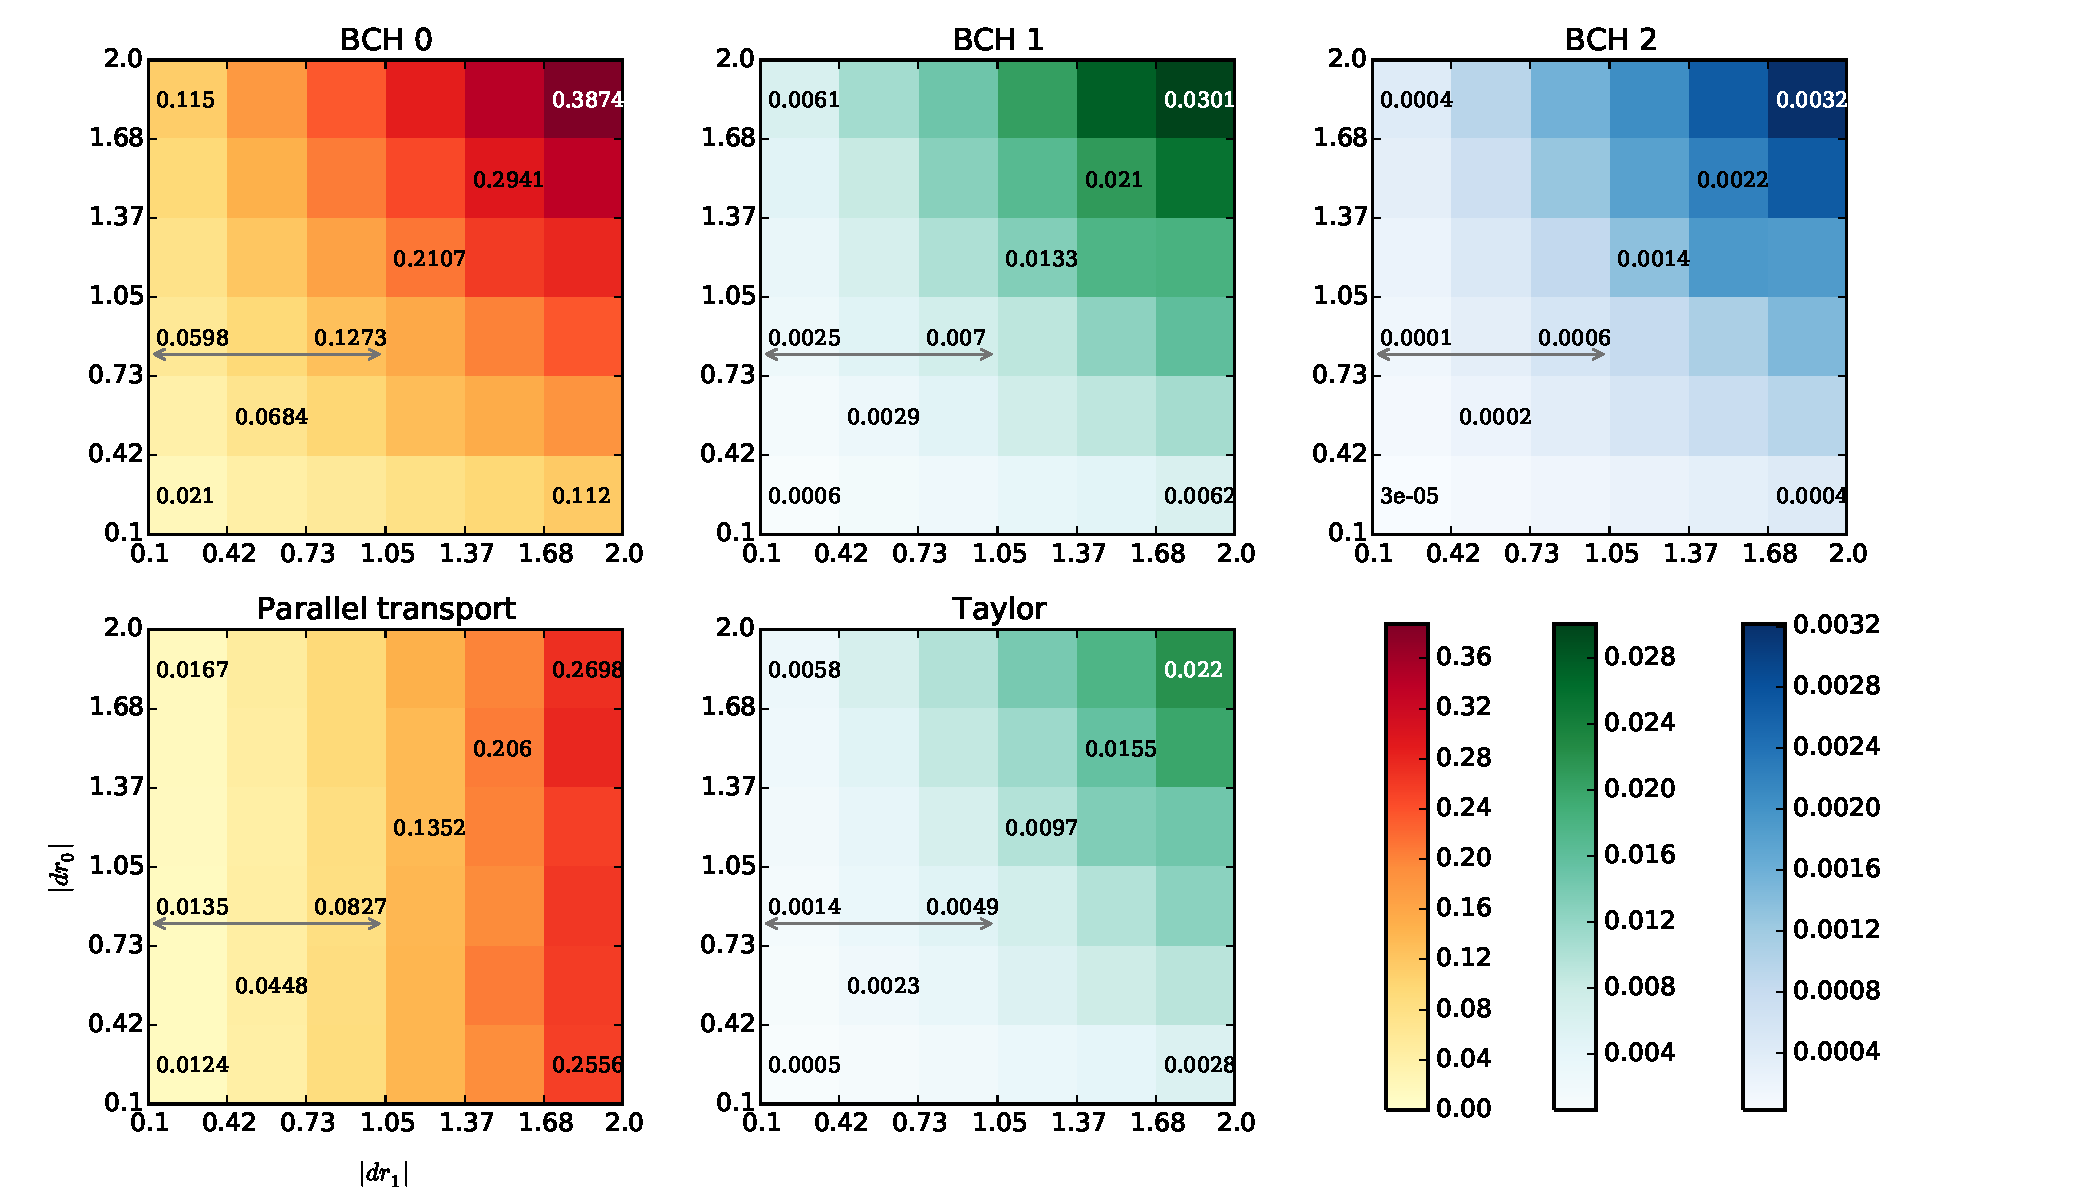
\includegraphics[scale=0.50]{figures/se2_image_scale.pdf}
 	\caption{Comparisons of the errors for each numerical method to compute the Log-composition $dr_{0} \oplus dr_{1}$ in $\mathfrak{se}(2)$. Truncated BCH of degrees 0,1,2, parallel transport method and Taylor method are considered for different values of the norm of $dr_{1}$ (x-axes) and norm of $dr_{0}$ (y-axes). 
 	The value of each square corresponds to the average error of 500 random samples in each of the 6 sub-intervals between $0.1$ and $2.0$. 
 	As expected errors increases with the norm for all of the methods.
 	Errors with BCH 0 and parallel transport method are comparable, but the parallel transport method is not symmetric and has better performance when $dr_{1}$ is small. $\text{BCH}^1$ and Taylor are comparable as well, and they are both symmetric, but the best performance is provided by the BCH 2. Details of the value under the \emph{gray arrows} are shown in the box-plot \ref{fig:se2_image_scale} where means, variance, range, quartiles and outliers are visualized.
 	 }
 	\label{fig:se2_image_scale}
 \end{figure}
 %
% % % % % % % % % % % % % % % % % % % % % % % % % % % % % % % % % % % % % %
% % % % % % % % % % % % % % % % % % % % % % % % % % % % % % % % % % % % % % 
\subsection{Methods and Results}

To compare the errors of the computation of the log-composition for the methods here presented, two sets of $3000$ transformations of elements in $\mathfrak{se}(2)$ are randomly sampled with increasing norms in the interval $[0.1, 2.0]$. Since the precision of the results is affected by the norm of the involved SVF, this interval is divided into 6 segments delimited by the values $I = [0.1, 0.42, 0.73, 1.05, 1.73, 1.68 ]$; choosing a couple of subintervals $[I(n_0), I(n_0+1)]$ and $[I(n_1), I(n_1+1)]$, two sets of $500$ transformations $\{ dr_{0}^{(j)}\}_{j=1}^{500}$, $\{ dr_{1}^{(j)} \}_{j=1}^{500}$ are sampled with norms belonging to the selected intervals:
\begin{align*}
j=1,...,500 \quad &\quad  n_0, n_1 = 0,...,5 \\
\euclideanMetric{dr_{0}^{(j)}}_{\text{fro}} &\in [I(n_0), I(n_0+1)] \\
\euclideanMetric{dr_{1}^{(j)}}_{\text{fro}} &\in [I(n_1), I(n_1+1)]  
\end{align*} 
If $M$ is one of the numerical methods presented in section \ref{se:rigid_body_transformations} for the computation of the log-composition - $\text{BCH}^{0}, \text{BCH}^{1}, \text{BCH}^{2}, \text{Taylor}, \text{p.t.}$ (parallel transport) - 
then the error between the ground truth and the approximation provided by one of these numerical methods is given by
\begin{align*}
\text{Error}(dr_{0},dr_{1},M) 
:= 
\euclideanMetric{dr_{0} \oplus dr_{1}
- 
M(dr_{0}, dr_{1}) }_{\text{fro}} 
\end{align*}

In figure \ref{fig:se2_image_scale}, each of the figure corresponds to a different method and each of the grade scale is the value computed with the function:
\begin{align*}
f(n_0,n_1,M) 
=
 \mathbb{E}\Big(
  \{ 
  \text{Error}(dr_{0}^{(j)},dr_{1}^{(j)}, M) 
  \}_{j=1}^{500}
  \Big)
\end{align*}
where the norm of $dr_{0}^{(j)}$ belongs to the interval $[I(n_0), I(n_0+1)]$ and the norm of 
$dr_{1}^{(j)}$ belongs to $[I(n_1), I(n_1+1)]$, and where $\mathbb{E}$ is the mean value.\\
The details for a chosen interval, indicated by the gray arrows in each plot, can be visualized in the box-plot \ref{fig:se2_boxplot}.
%
\begin{figure}[!ht]
	\hspace{-1cm}
	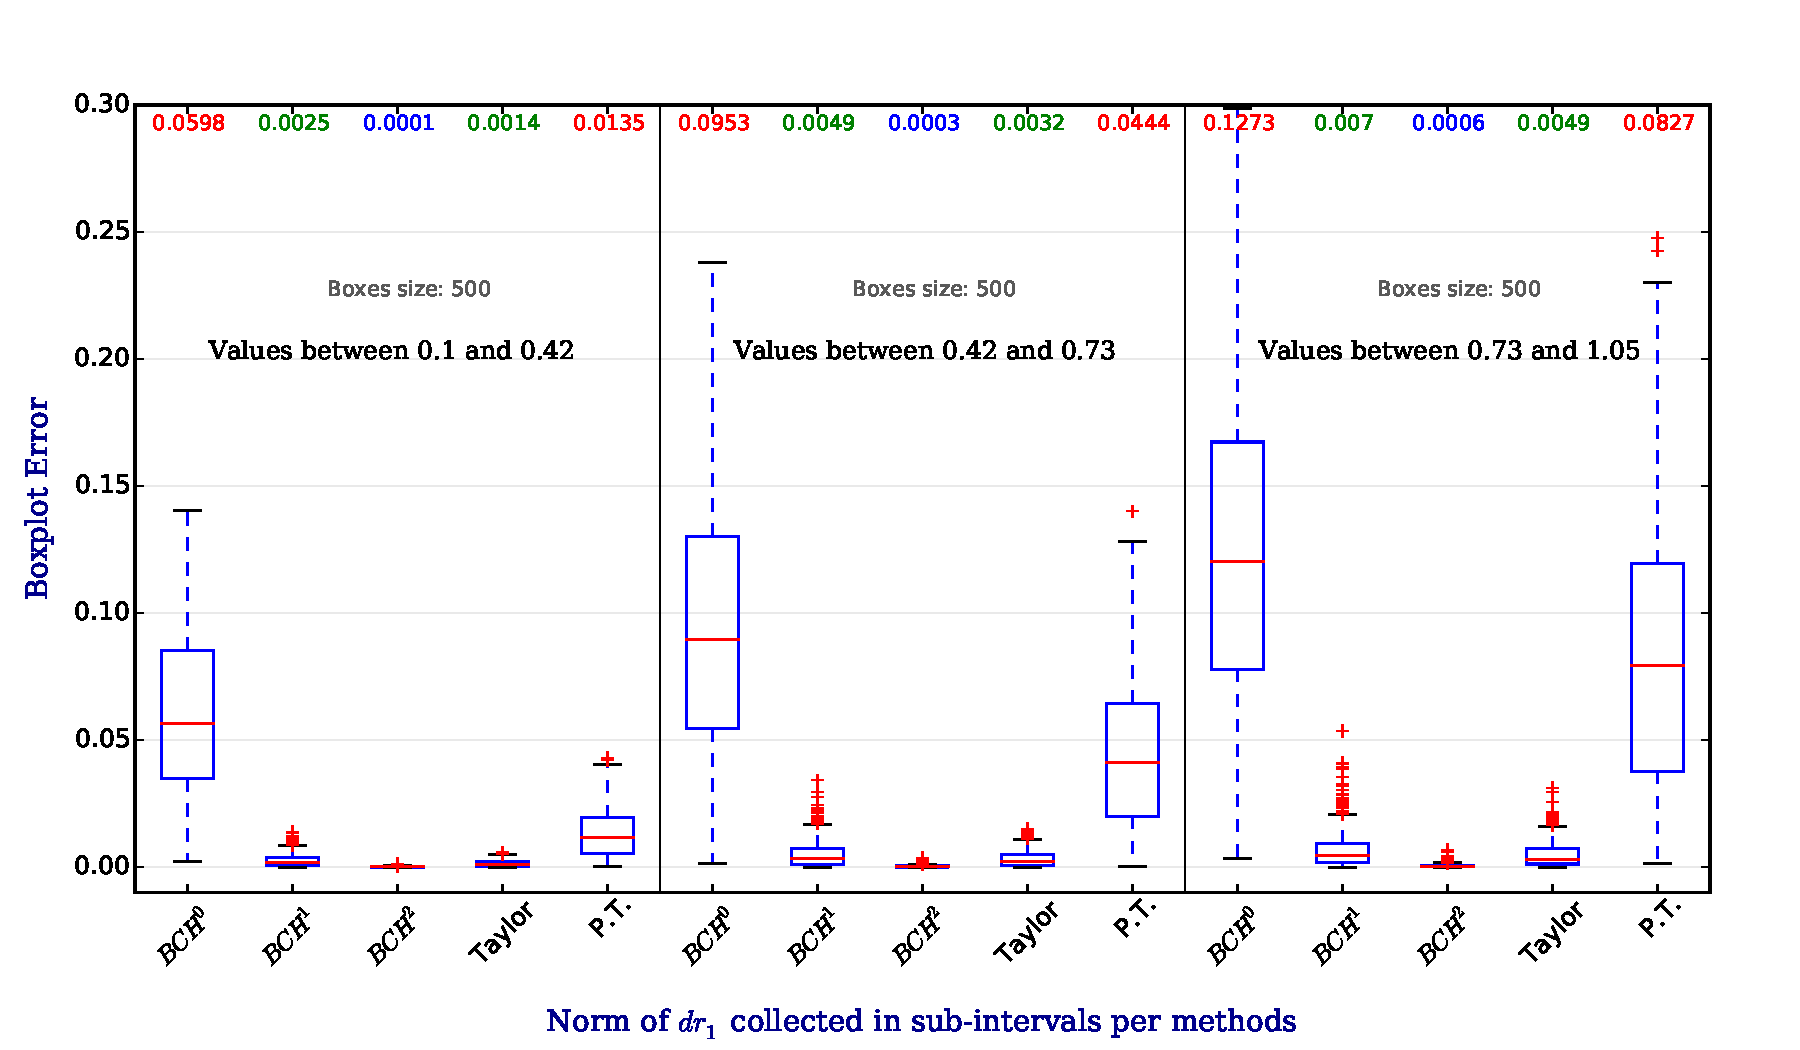
\includegraphics[scale=0.51]{figures/se2_boxplot.pdf}
	\caption{Errors of the numerical methods for the computation of the Lie log-composition of $dr_{0} \oplus dr_{1}$ in $\mathfrak{se}(2)$. Norm of $dr_{0}$ is in the interval $[0.37,1.05]$, norm of $dr_{1}$ in the interval $[0.1, 1.05]$ divided in 3 segments: $[0.1,0.42] $, $[0.42, 0.73] $, $[0.73, 1.05] $. Mean values of each box are shown in the first row in different colors. Shown data corresponds to a section of the image scale \ref{fig:se2_image_scale}, indicated by a gray arrow. As expected all of the error means increase with the of norm of $dr_1$, but the rate of growth is different for each method.}
	\label{fig:se2_boxplot}
\end{figure}
%

The method based on the $BCH^0$ provides the worst results. It does not involves any Lie bracket and so it does not take into account the geometrical curvature of the Lie group. Parallel transport method tries to compensate the curvature using a geometrical approach. As expected from the formula, and as it can be seen clearly in the image scale, it is not a symmetric method. It provides better results than the $BCH^0$; for small norm of $dr_1$, results are close to the one obtained with $BCH^1$ when norms of $dr_0$ and $dr_1$ are below $1.3$.

Lie log-composition based on Taylor method has slightly better results than the $BCH^1$, but do not reach $BCH^2$, which provides the best results. This may be due to the fact that the Taylor method belongs to $\mathcal{O}(dr_1^2)$ while the $BCH^2$ involves the Lie bracket $[dr_0,[dr_0, dr_1]] + [dr_1,[dr_1, dr_0]]$. Even if the truncated $BCH$ does not have a known asymptotic error (or big-O notation), we can see experimentally that $BCH^2$ have a larger asymptotic order of converges than $\mathcal{O}(dr_1^2)$, in $\mathfrak{se}(2)$.
%
\begin{figure}[!ht]
	%\hspace{0cm}
	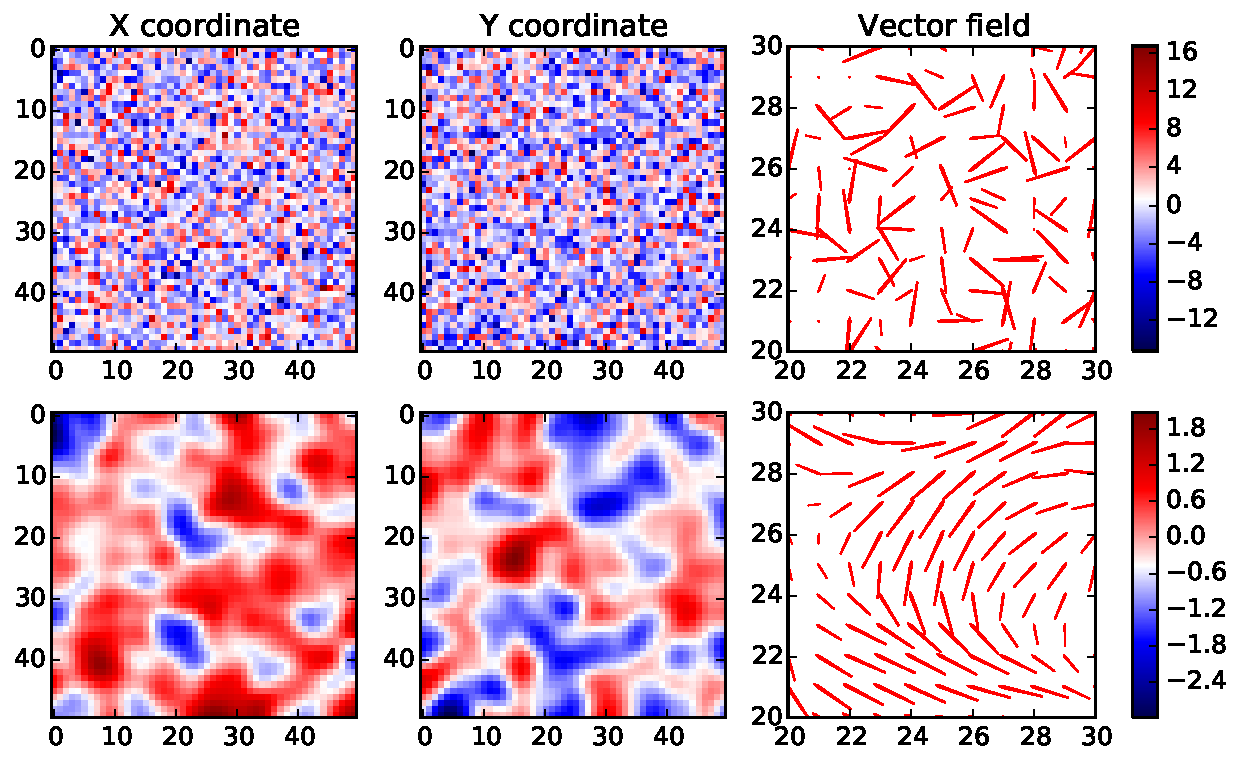
\includegraphics[scale=0.70]{figures/svf_gaussian_smoothing_effects.pdf}
	\caption{Random generated vector field before and after the Gaussian smoother. In the first row is shown a random generated vector field of dimension $50\times 50 \times 2$. Values of the vectors at each pixel are sampled from a random variable with normal distribution of mean $0$ and sigma $4$. The second row shows the same random vector field after a Gaussian smoothing of sigma $2$ (the code is based on the scipy library ndimage.filters.gaussian\textunderscore filter). The last column shows the quiver of the vector field in the squared subregion of size $10\times 10$ at the point $(20,20)$. From the colorscale it is also possible to see that the values distribution of the filtered image have lost their symmetry. }
	\label{fig:SVF_gaussian_smoothing_effects}
\end{figure}

% % % % % % % % % % % % % % % % % % % % % % % % % % % % % % % % % % % % % %
% % % % % % % % % % % % % % % % % % % % % % % % % % % % % % % % % % % % % %
% % % % % % % % % % % % % % % % % % % % % % % % % % % % % % % % % % % % % % 
% % % % % % % % % % % % % % % % % % % % % % % % % % % % % % % % % % % % % % 
\section{Log-composition for SVF}
Before getting into the results for the Lie log-composition of SVF we show how random SVF are created and, in particular, how the norm of the approximation of $\mathbf{u}_0\oplus \mathbf{u}_1$ is compared with the ground truth when this is not directly available.

% % % % % % % % % % % % % % % % % % % % % % % % % % % % % % % % % % % % % %
% % % % % % % % % % % % % % % % % % % % % % % % % % % % % % % % % % % % % % 
\subsection{Methods: random generated SVF}
% How to generate a random SVF
A random generated SVF is a $5$-dimensional matrix with the structure presented in the formula (\ref{eq:basic_data_structure}). 
The vectors at each point of the grid are generated in two phases. 
In the first one, the values of the coordinates of the vectors are randomly sampled from a normal distribution of mean zero and standard deviation $\sigma_{\text{init}}$. 
In the second phase vectors are smoothed with a Gaussian filter with standard deviation $\sigma_{\text{gf}}$. In figure \ref{fig:SVF_gaussian_smoothing_effects} it is possible to see the effects of the two phases on a bi-dimensional $50\times 50$ image.

\begin{figure}[!ht]
	\hspace{-1cm}
	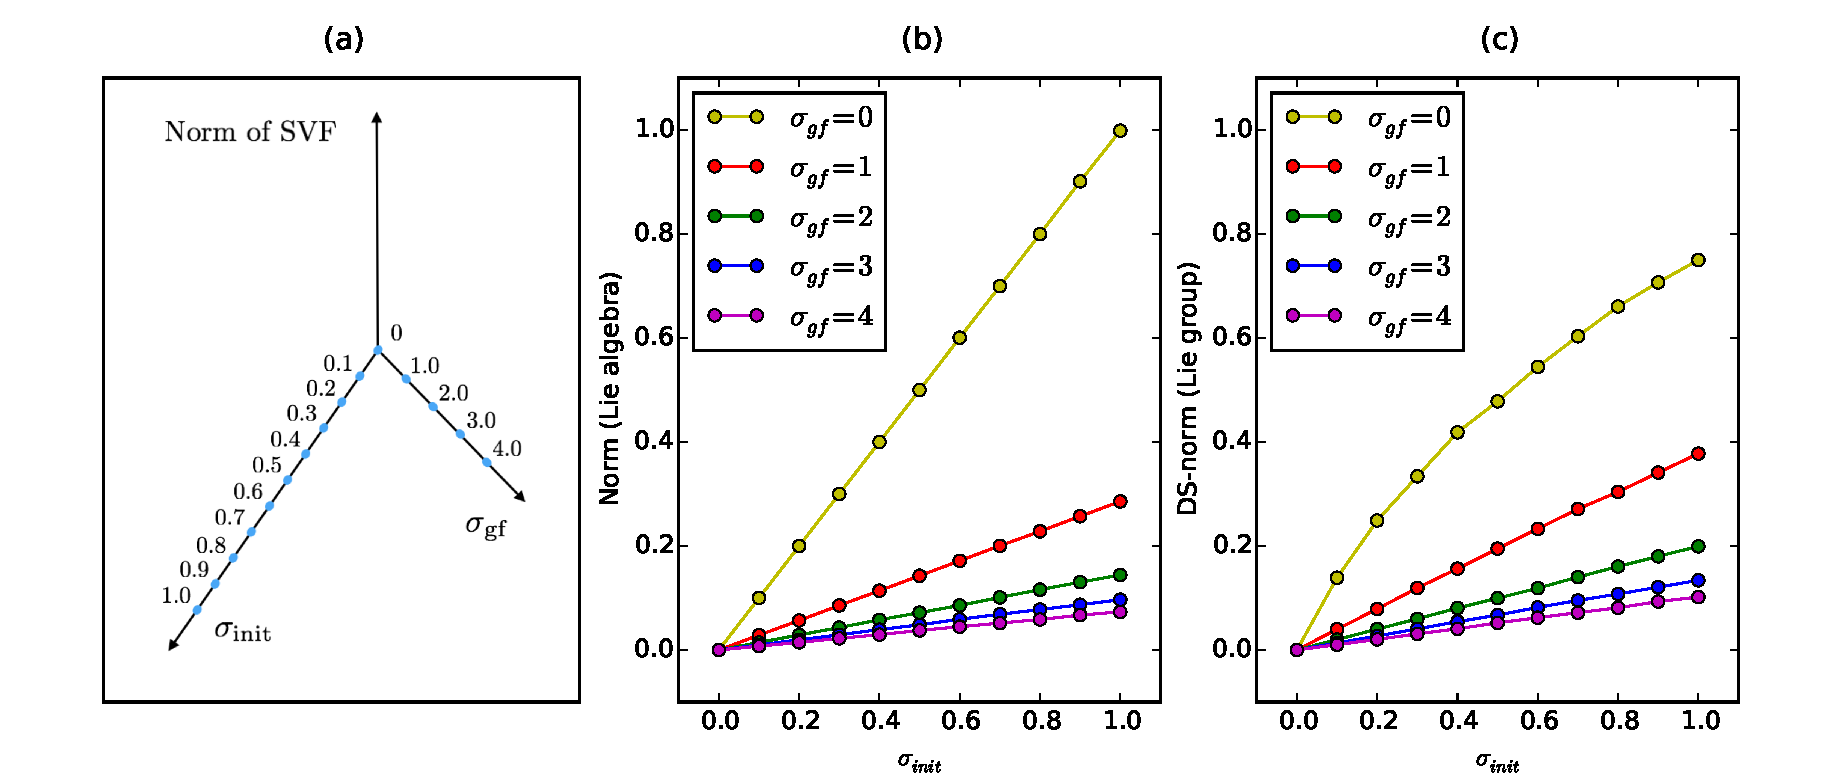
\includegraphics[scale=0.51]{figures/SVF_sigma_means_comparisons.pdf}
	\caption{Relationships between the initial standard deviation $\sigma_{\text{init}}$ that defines the random SVF (stationary velocity field), the standard deviation of the Gaussian filter $\sigma_{\text{gf}}$ utilized to regularize the SVF and its norm. Figure (a) represents schematically the two factors that define the norm of an SVF and with the blue dots we emphasized the values that has been chosen for the numerical computations proposed in (b) and (c). Figure (b) shows the mean of the norm of $10$ random generated SVF, with initial standard deviation $\sigma_{\text{init}}$ (on the x-axis) and Gaussian filter with standard deviation $\sigma_{\text{gf}}$ (in different colors).
		Figure (c) shows the norm of the same element after exponentiating and so after having them in the Lie algebra.
		It is important to remark that it is not possible in general define a norm on a group. Nevertheless for matrices and for SVF it is possible to extend the norm from the Lie algebra to the Lie group, as proposed in chapter \ref{ch:spatial_transformations} with the definition of displacement field norm (DS-norm) proposed in equation (\ref{eq:ds_norm}). }
	\label{fig:SVF_sigma_means_comparisons}
\end{figure}

% Norm defined in both Lie algebra and Lie group
After discretization, the norm of an SVF can be computed from the discretized version of the metric presented in equation (\ref{def:metric_two_svf}). The norm $l^2$ is considered instead of $L^2$ and $\Delta\Omega$, discretization of the domain, substitutes $\Omega$:
\begin{align*}
\euclideanMetric{\mathbf{u}}  
= 
\Big( \sum_{\mathbf{x} \in \Delta\Omega} \euclideanMetric{\mathbf{u}(\mathbf{x}) }_{l^2}^{2}  \Big)^{1/2}
\end{align*} 
This norm coincides with the Frobenius Norm of the $5$-dimensional matrices $\mathbf{u}$.
When an SVF $\mathbf{u}$ is exponentiated in the Lie algebra, $\exp(\mathbf{u}) = \varphi$, we can rely on the fact that $\varphi - 1$ is a vector field whose norm can be computed with the discretization of the metric presented in equation (\ref{def:metric_two_displacement_field}):
\begin{align}\label{eq:ds_norm}
\euclideanMetric{\varphi}  
= 
\Big( \sum_{\mathbf{x} \in \Delta\Omega} \euclideanMetric{\mathcal{V}(\varphi)(\mathbf{x}) }_{l^2}^{2}  \Big)^{1/2}
=
\Big( \sum_{\mathbf{x} \in \Delta\Omega} \euclideanMetric{\varphi(\mathbf{x}) - \mathbf{x} }_{l^2}^{2}  \Big)^{1/2}
\end{align} 
To distinguish the norm of the SVF from the norm of the vector field associated to its exponential, we call the latter DS-norm (displacement norm); as before, it coincides with the Frobenius norm of the $5$-dimensional matrices $\varphi - I$.

% Norm influenced by sigmas
We can see how these two norms are related in figure \ref{fig:SVF_sigma_means_comparisons}. The initial standard deviations $\sigma_{\text{init}}$ that defines the SVF are related with their norm before and after the exponentiation for $5$ different choices of the value of the standard deviation of the Gaussian filter $\sigma_{\text{gf}}$.
For the extreme case $\sigma_{\text{gf}} = 0$, where the SVF is not properly defined, the norm after the exponentiation does not maintain linearity, but in all the other cases an element in the Lie algebra $\mathbf{u}$ increases the norm after the exponentiation. Moreover, for a fixed $\sigma_{\text{gf}} $ in both algebraic structures the norms shows a linear trend with the increase of $\sigma_{\text{init}}$. An increase in $\sigma_{\text{gf}} $ implies a decrease in the slope of the linear model.

% Slopes formulae
The linear regression of the model for each $\sigma_{\text{gf}}$ are given, in Cartesian coordinate by:
\begin{align}\label{eq:angular_coefficients_for_the_gf}
y = m_{\text{alg}}( \sigma_{\text{gf}} )x \qquad  \sigma_{\text{gf}} \geq 0
\qquad
\qquad
y = m_{\text{grp}}( \sigma_{\text{alg}} )x \qquad  \sigma_{\text{alg}} \ge 0
\end{align}
Where we indicated with $m_{\text{alg}}$ and $m_{\text{grp}}$ angular coefficients for the results obtained in the Lie algebra and in the Lie group respectively (figure \ref{fig:SVF_sigma_means_comparisons} (b) and (c)). They follow an exponential model, given by
\begin{align}
m_{\text{alg}}( \sigma_{\text{gf}} )
=
\alpha_0 e^{-\beta_0 \sigma_{\text{gf}}} + \gamma_0 
\qquad
m_{\text{grp}}( \sigma_{\text{gf}} )
=
\alpha_1 e^{-\beta_1 \sigma_{\text{gf}}} + \gamma_1
\end{align}
Where the parameters $\alpha_i, \beta_i, \gamma_i$ for $i=1,2$ can be computed numerically using an exponential regression algorithm:
\begin{center}
	\begin{tabular}{ c | c |c |c |c |c}
	$\alpha_0$ & $\beta_0$ & $\gamma_0$ & $\alpha_1$ & $ \beta_1$ & $\gamma_1$ \\
	\hline
	0.91422836 &  1.48548466 &  0.08393943 &  0.67302265 &  0.82680977 &  0.07765811
	\end{tabular}
\end{center}

These values are useful when, given two values among $\sigma_{\text{init}}$, $\sigma_{\text{gf}}$ and the $\euclideanMetric{\mathbf{u}}$, we want to know the third one.

% Conclusion for the presentation of the random SVF
After showing how a random SVF is generated by the parameters $\sigma_{\text{init}}$ and $\sigma_{\text{gf}}$, and what is the relationship between the parameters and the resulting norm in both Lie algebra and Lie group, we can move toward the results of the numerical method for the Lie log-composition obtained with these objects.

\begin{figure}[!ht]
	\hspace{-2.1cm}
	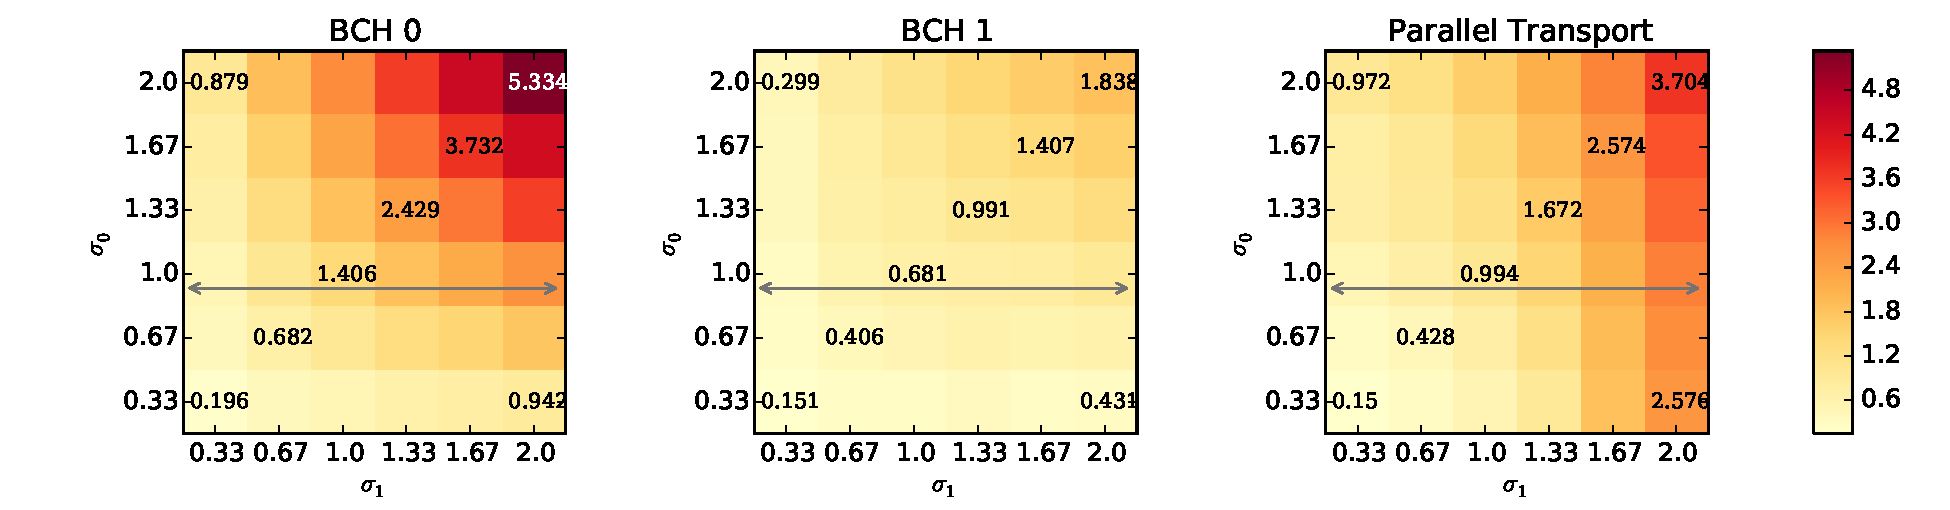
\includegraphics[scale=0.55]{figures/SVF_image_scale.pdf}
	\caption{Mean errors for the numerical computation of the Log-composition of randomly generated stationary velocity fields (SVF). Initial standard deviations of the SVF $\sigma_{\text{init}}^{0}$ and $\sigma_{\text{init}}^{1}$ are given by the values on the axis for each sampling of $15$ elements. The error is computed using the formula (\ref{eq:error_svf_sythetic_data}). When the norm of $\mathbf{u}_1$ is small (see figure \ref{fig:SVF_sigma_means_comparisons} to infer the norm from the standard deviations), parallel transport method and truncated BCH of degree 1 have comparable results, but parallel transport, as expected from the formula, is not symmetric respect to the size of the input vectors. Results of another sampling with the value of $\sigma_{\text{init}}^{0}$ and $\sigma_{\text{init}}^{1}$ are shown in figure \ref{fig:SVF_scatter_plot}. The reason why results obtained $\text{BCH}^{1.5}$ and $\text{BCH}^{2}$ is presented in figure \ref{fig:SVF_boxplot_comparisons_BCH}.}
	\label{fig:SVF_image_scale}
\end{figure}

\begin{figure}[!ht]
	\hspace{-1.5cm}
	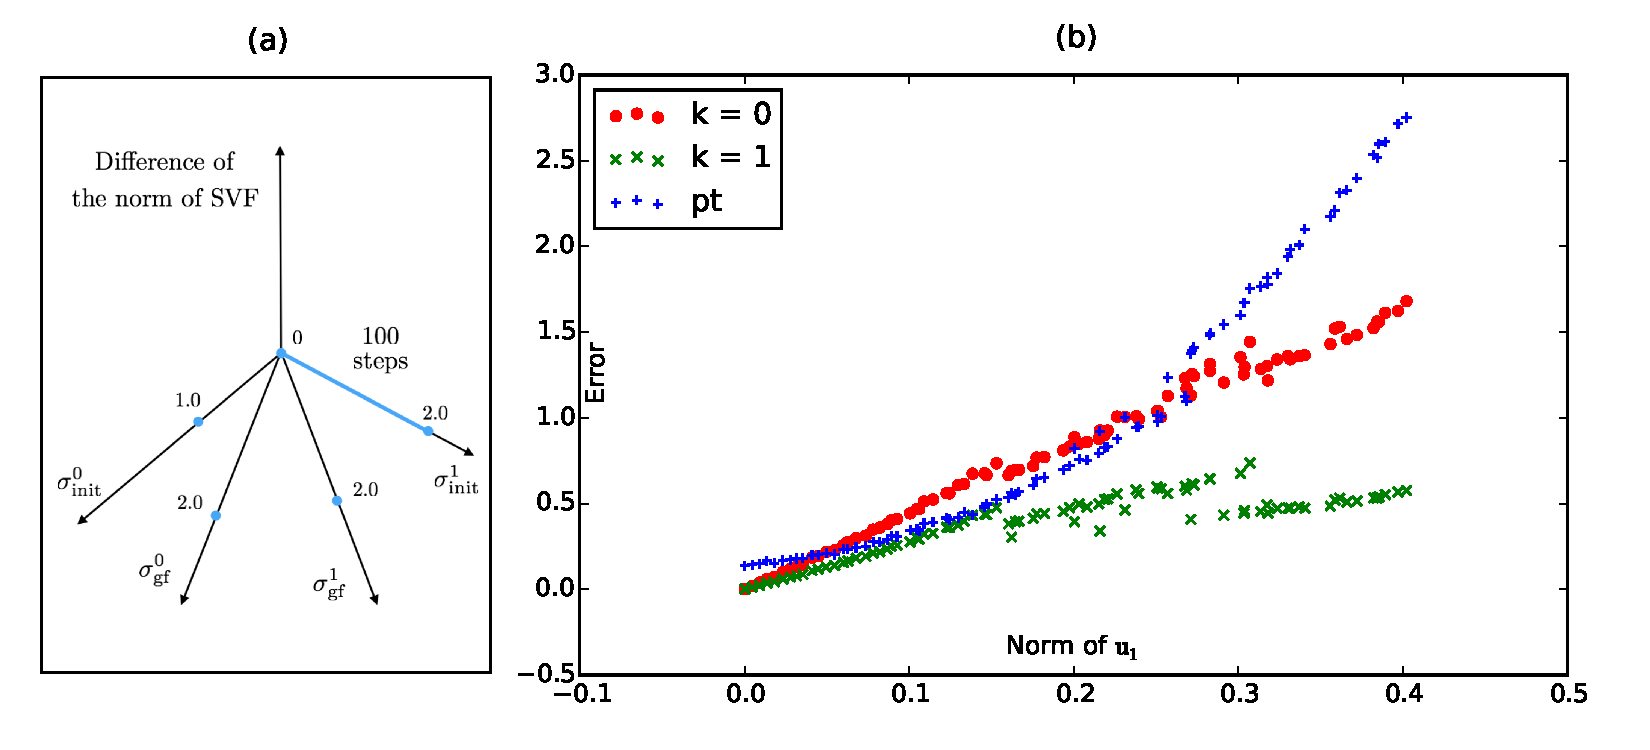
\includegraphics[scale=0.6]{figures/SVF_scatter_plot.pdf}
	\caption{Comparisons of the errors of numerical computations of the Lie log-composition $\mathbf{u}_0\oplus \mathbf{u}_1$ with the method of truncated BCH of degree 0,1 and parallel transport. Parameters' values of the random generated SVF are schematically represented in figure (a). A set of $90$ SVF $\mathbf{u}_0$ are generated with fixed parameters $\sigma_{\text{gf}}^{0} = 2.0$ and $\sigma_{\text{init}}^{0} = 1.0$; a second set of $90$ SVF  $\mathbf{u}_1$, are generated with the parameters $\sigma_{\text{gf}}^{1} = 2.0$ and $\sigma_{\text{init}}^{1}$ uniformly scattered in the the interval $(0.0, 2.0)$. On the x-axis fo figure (b) is shown the value of the resulting norm of $\mathbf{u}_1$ for the chosen parameters, while on the y-axes are shown the values of the error for the numerical computation of the Log-composition $\mathbf{u}_0\oplus \mathbf{u}_1$ for each of the chosen methods.  }
	\label{fig:SVF_scatter_plot}
\end{figure}
%\begin{figure}[!ht]
%	\hspace{-1.5cm}
%	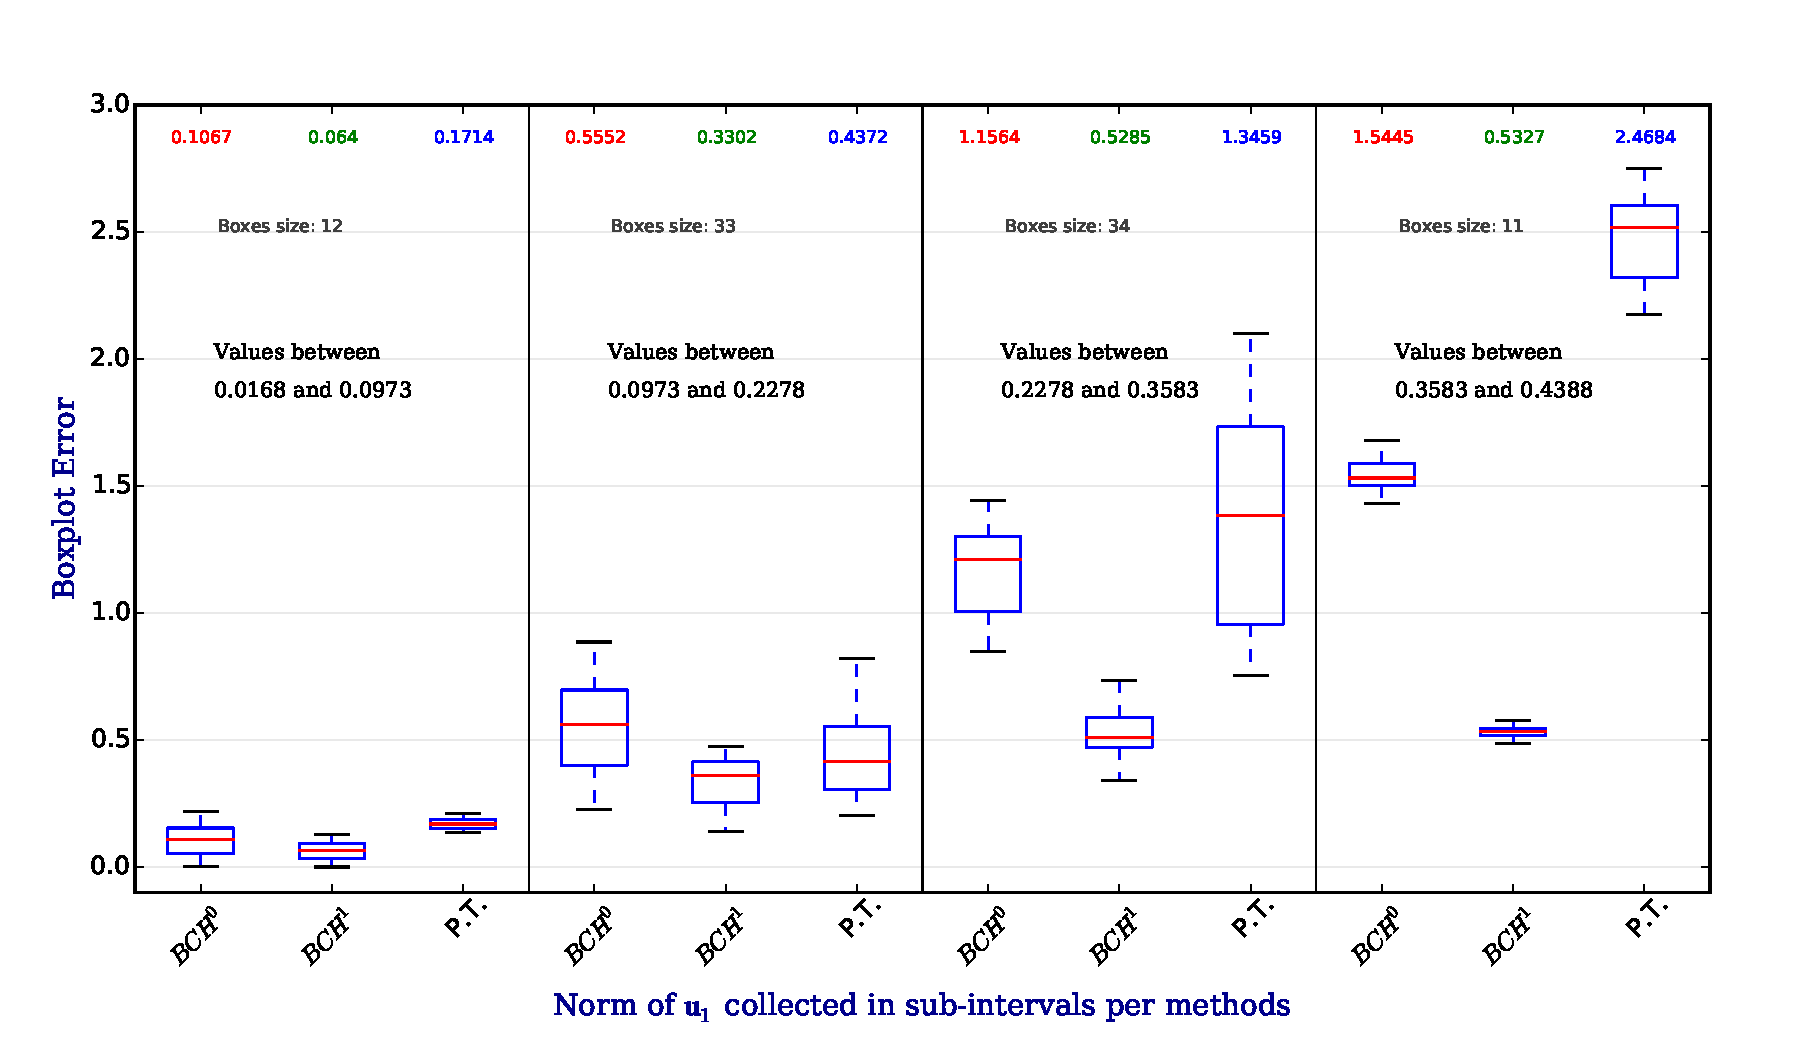
\includegraphics[scale=0.5]{figures/SVF_boxplot.pdf}
%	\caption{Log-composition for SVF computed using numerical methods of truncated BCH of degree 0,1 and parallel transport, represented in a boxplot.}
%	\label{fig:SVF_boxplot}
%\end{figure}

% % % % % % % % % % %% % % % % % % % % % %
% % % % % % % % % % %% % % % % % % % % % % % % % % % % % % % %
\subsection{Lie Log-composition for synthetic SVF}
% which norm?
This section shows the results of the numerical computation of the Lie log-composition $\mathbf{u}_0\oplus\mathbf{u}_1 = \log(\exp(\mathbf{u}_0)\circ \exp(\mathbf{u}_1))$ when $\mathbf{u}_0$ and $\mathbf{u}_1$ are synthetic SVF. Despite the lack of a ground truth for the SVF it is reasonable to compare the numerical approximation of the exponential of $\mathbf{u}_0\oplus\mathbf{u}_1$ with $\exp(\mathbf{u}_0)\circ \exp(\mathbf{u}_1)$. The norm utilized is the one proposed in the equation 9\ref{def:metric_one_svf_one_displacement_field}):
\begin{align}
\text{Error}_{\oplus}(\mathbf{u}_0, \mathbf{u}_1)
= 
\Big(\int_{\Omega} \euclideanMetric{\mathcal{V}(\exp(\mathbf{u}_0\oplus\mathbf{u}_1)) - \mathcal{V}(\exp(\mathbf{u}_0)\circ \exp(\mathbf{u}_1))}_{L^2}^{2} d\mathbf{x} \Big)^{1/2}
\end{align} 
that, when discretized becomes
\begin{align}\label{eq:error_svf_sythetic_data}
\text{Error}_{\oplus}(\mathbf{u}_0, \mathbf{u}_1) 
= 
\Big( \sum_{\mathbf{x} \in \Delta\Omega} 
\euclideanMetric{\exp(\mathbf{u}_0\oplus\mathbf{u}_1)(\mathbf{x}) 
	-
\big(\exp(\mathbf{u}_0)\circ \exp(\mathbf{u}_1)\big)(\mathbf{x}) 
	  }_{l^2}^{2}  \Big)^{1/2}
\end{align} 
For the unknown analytical result of $\mathbf{u}_0\oplus\mathbf{u}_1$ the error of the above equation is $0$, since $\exp(\mathbf{u}_0\oplus\mathbf{u}_1)$ $=$
$\exp(\mathbf{u}_0)\circ \exp(\mathbf{u}_1)$. When we use one of the introduced numerical method we obtain the results presented in figure \ref{fig:SVF_image_scale} and \ref{fig:SVF_scatter_plot}. 

The limitation of this strategy to compute the error of the numerical method without a ground truth is that it is based on the numerical algorithm utilized for the computation of the Lie exponential (the scaling and squaring in this experiment \cite{arsigny2006log}). But this limitation tend to not bias the results, since scaling and squaring is utilized it the both sides of the difference in the computation of the error.

% figures presentation and comment to general results.
In figure \ref{fig:SVF_image_scale}, we can see the differences between the errors obtained with the numerical methods based on $\text{BCH}^0$, $\text{BCH}^1$ and parallel transport. To each square corresponds the mean of $15$ log-compositions between the SVF $\mathbf{u}_0$ and $\mathbf{u}_1$ randomly generated. The parameters $\sigma_{\text{init}}^{0}$ and $\sigma_{\text{init}}^{1}$ are equals to one of the value in the array $(0.33, 0.67, 1, 1.33, 1.37, 2.0)$ while the standard deviation of the Gaussian filter $\sigma_{\text{gf}}^{0}$ and $\sigma_{\text{gf}}^{1}$ are constant and equal to $2.0$. As previously noticed for matrices, the methods based on the truncated  BCH are symmetric while the same does not happen for the parallel transport. 

The SVF in the subinterval indicated by the gray arrow on the figure \ref{fig:SVF_image_scale} are shown in figure \ref{fig:SVF_scatter_plot}, where the values of $\mathbf{u}_1$ are equally distributed. From there we can see that parallel transport works better than the $\text{BCH}^0$ only when the norm of $\mathbf{u}_1$ is small enough.

% introduction of the next section
In the results just shown there is a notable absent: the numerical computation of the Lie log-composition based on truncated BCH of order greater than $1$. The next section explains why, and in particular why we are interested in BCH-free numerical methods for the log-composition, as the one based on parallel transport.


% % % % % % % % % % % % % % % % % % % % % % % % % % % % % % % % % % % % % %
% % % % % % % % % % % % % % % % % % % % % % % % % % % % % % % % % % % % % % 
\subsection{Truncated BCH formula: The problem of the Jacobian matrix.}\label{se:jacobian_problem}

% why we will take into account only the BCH 0 and the BCH 1 methods.
% Theoretical problems: that the Jacobian is utilized in the Lie bracket from Marcos' paper
As shown in figure \ref{fig:se2_image_scale}, for the finite dimensional case, the truncated BCH of degree $2$ provides the best results over the Taylor method and the parallel transport method.

We would expect something similar for SVF, but in this case the use of the truncated BCH of degree greater than $1$ is problematic, because Jacobian matrices are involved.

\begin{figure}[!ht]
	\hspace{0cm}
	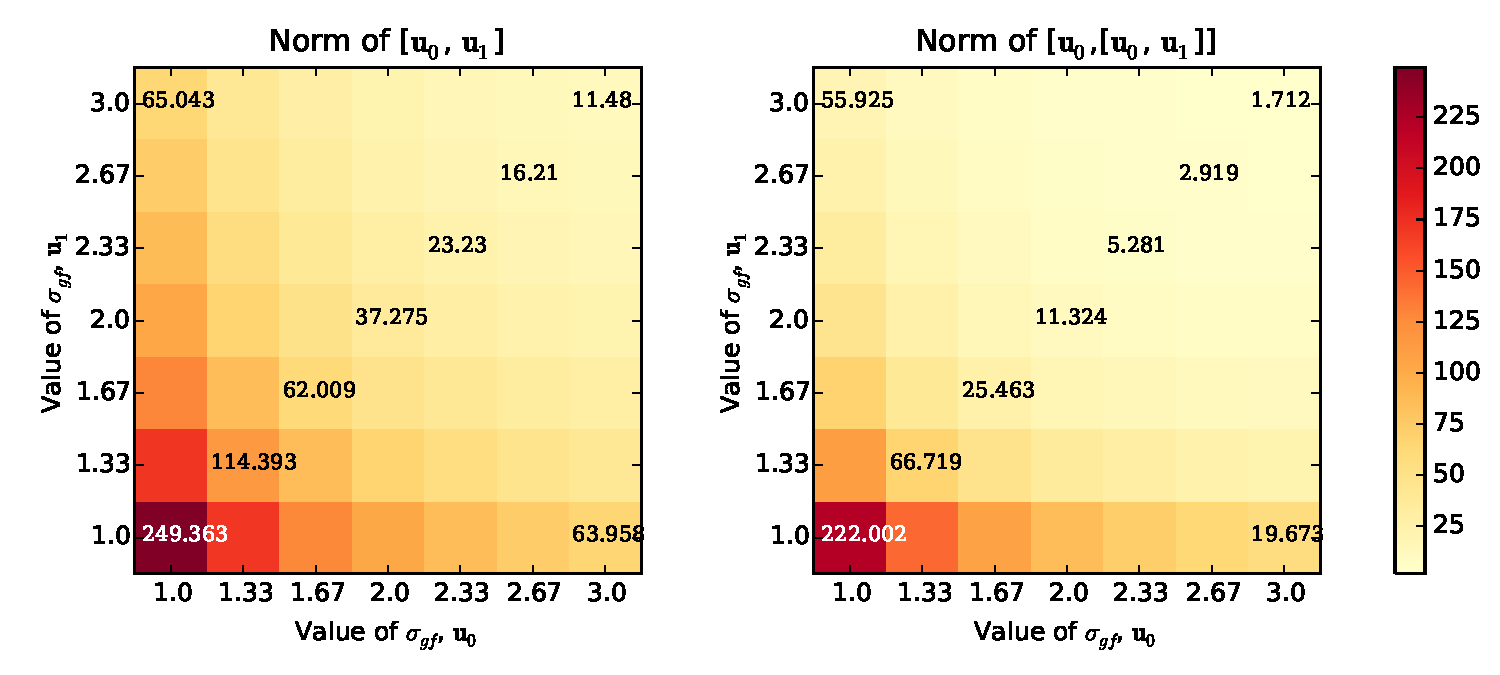
\includegraphics[scale=0.5]{figures/SVF_image_scale_bracket_versus_gaussian.pdf}
	\caption{Relationships between the standard deviation of the Gaussian smoother that generates the SVF and the norm of the Lie bracket. Each square contains the means of $10$ Lie bracket (left) or nested Lie bracket (right) generated with initial standard deviation equals to $2$ and standard deviation of the gaussian smoother $\sigma_{\text{gf}}$ indicated on the axes.}
	\label{fig:SVF_image_scale_bracket_versus_gaussian}
\end{figure}

% 2 limitation of the JACOBIAN. Image scale figure
On one side, every time the differentiation of a vector is required, results are unstable and sensitive to noise, because of the finite difference method utilized for the numerical approximation. On the other side, in figure \ref{fig:SVF_image_scale_bracket_versus_gaussian} we can see that the smoother are the SVF the smaller is the norm of resulting Lie brackets. In consequence of this, for a couple of \lq\lq very smooth\rq\rq~ stationary velocity field, the higher term of the BCH carry small information extremely sensitive to noise.

% Boxplot comment, why it behave in this way 
The boxplot in figure \ref{fig:SVF_boxplot_comparisons_BCH} shows that an increase in the degree of the truncated BCH does not necessarily imply better results, in particular when the involved SVF have been generated with a small Gaussian smoother.

\begin{figure}[!ht]
	\hspace{-0.5cm}
	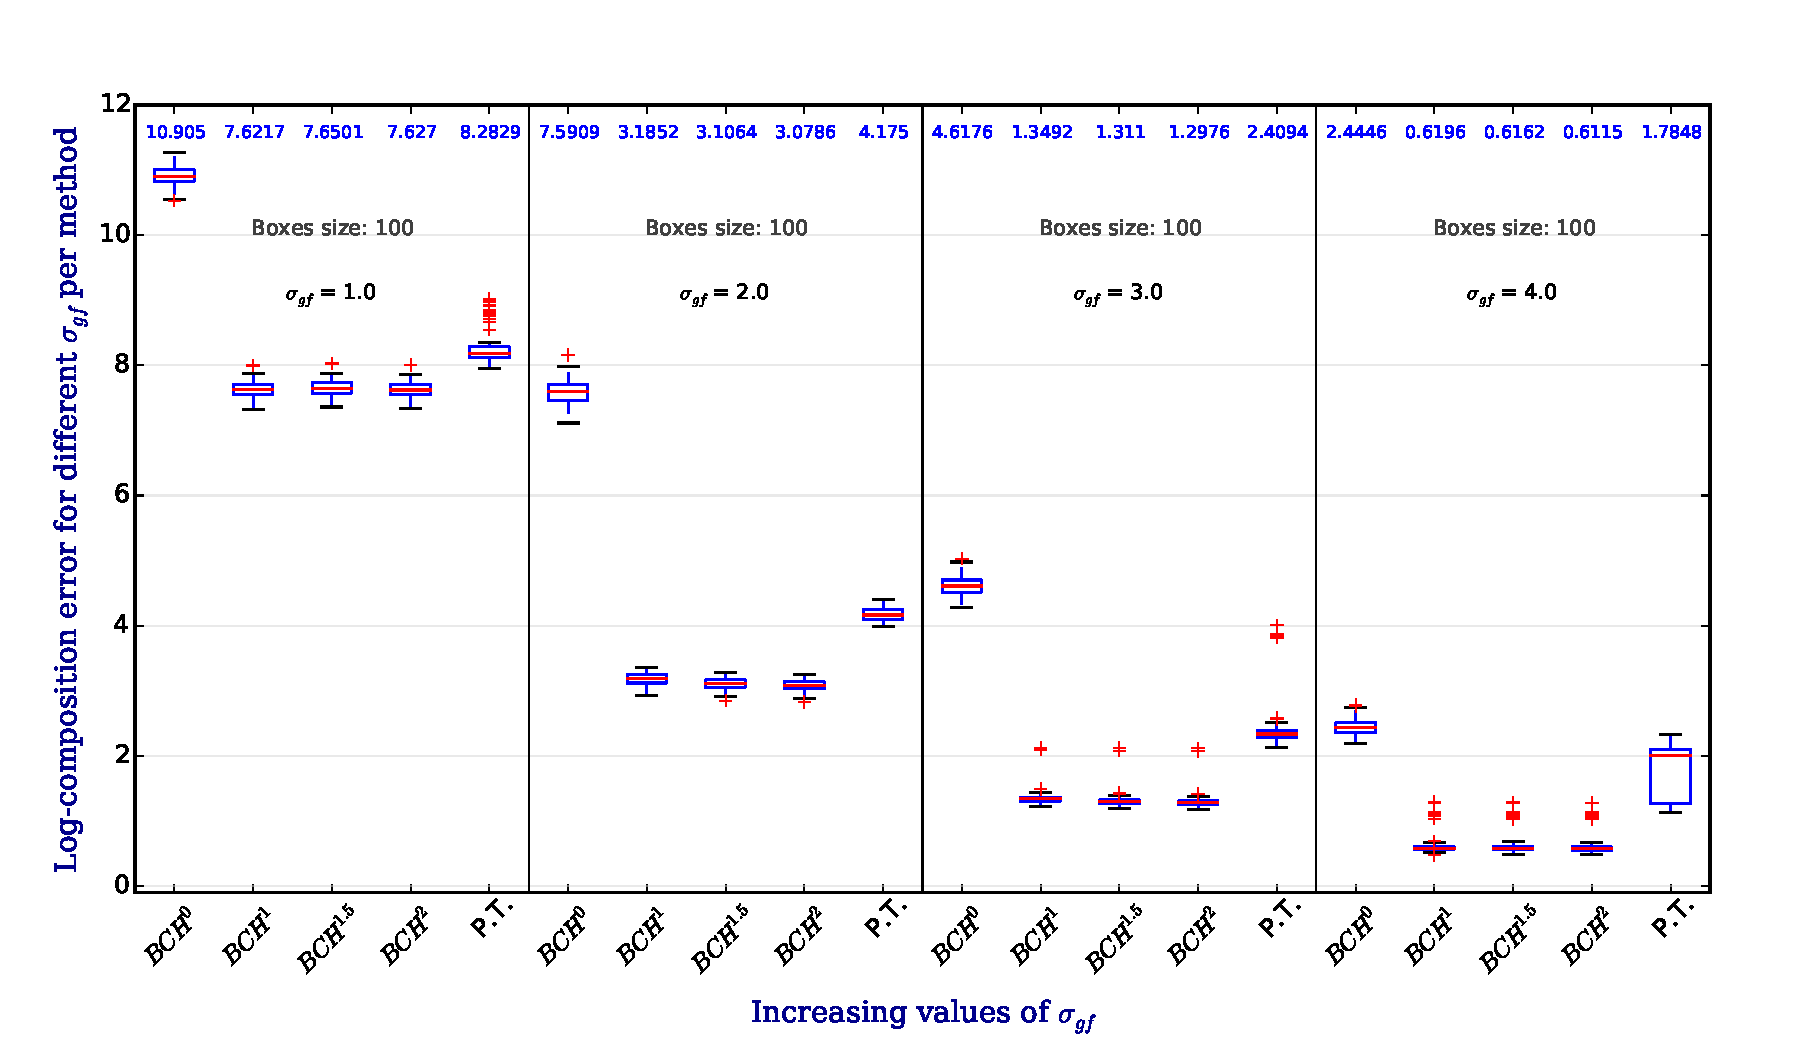
\includegraphics[scale=0.5]{figures/SVF_boxplot_comparisons_BCH.pdf}
	\caption{Boxplot to compare the error between truncated BCH methods of degree $0$, $1$, $1.5$ and $2$. The size of each box is $100$ and the approximation of $\mathbf{u}_{0}\oplus \mathbf{u}_1$ is performed with $\euclideanMetric{\mathbf{u}_{0}} = 1.0$ and $\euclideanMetric{\mathbf{u}_{0}} = 0.1$. The standard deviation of the Gaussian filter $\sigma_{\text{gf}}$ belongs to the set $(1.0, 2.0, 3.0, 4.0)$ and the initial standard deviation is computed such that $\sigma_{\text{init}} = \euclideanMetric{\mathbf{u}}/m_{\text{alg}}(\sigma_{\text{gf}})$ according to the formula (\ref{eq:angular_coefficients_for_the_gf}). With this strategy we have been able to compare vector of constant norm generated with increasing values for $\sigma_{\text{gf}}$. The numbers written in blue above each boxes represents the mean value of the errors. For small $\sigma_{\text{gf}}$, an increase in the order of the approximation does not always corresponds to a decrease in the error, and in general there no great improvements can be registered when the degree is greater than 1. }
	\label{fig:SVF_boxplot_comparisons_BCH}
\end{figure}


\newpage
% Conclusions for syntetic data: where are the errors and why we are moving towards the real data.
% Why going toward real svf, 

% % % % % % % % % % % % % % % % % % % % % % % % % % % % % % % % % % % % % %
% % % % % % % % % % % % % % % % % % % % % % % % % % % % % % % % % % % % % % 
\section{A Problem for Three Brains}\label{se:three_brains} % {A three-brain problem}
The experiments performed on synthetic data provide important informations to validate and compare the methods, but do not give informations about what may happen for real cases. 

To validate the method for real cases, one of the possibility is to embed the method in a diffeomorphic demon registration algorithm and compare the results obtained with different numerical methods of the Lie log-composition to compute the update.

But, since computation of the update is only a small component of the registration algorithm, it may be difficult to compute the impact of the Lie log-composition over other components that play a more important role in the registration algorithm (as the optimization strategy).

For this reason we chose to validate the numerical methods for the log-composition using the same strategy utilized for synthetic data, using SVF from longitudinal patient scans.

\begin{figure}[!ht]
	\centering
	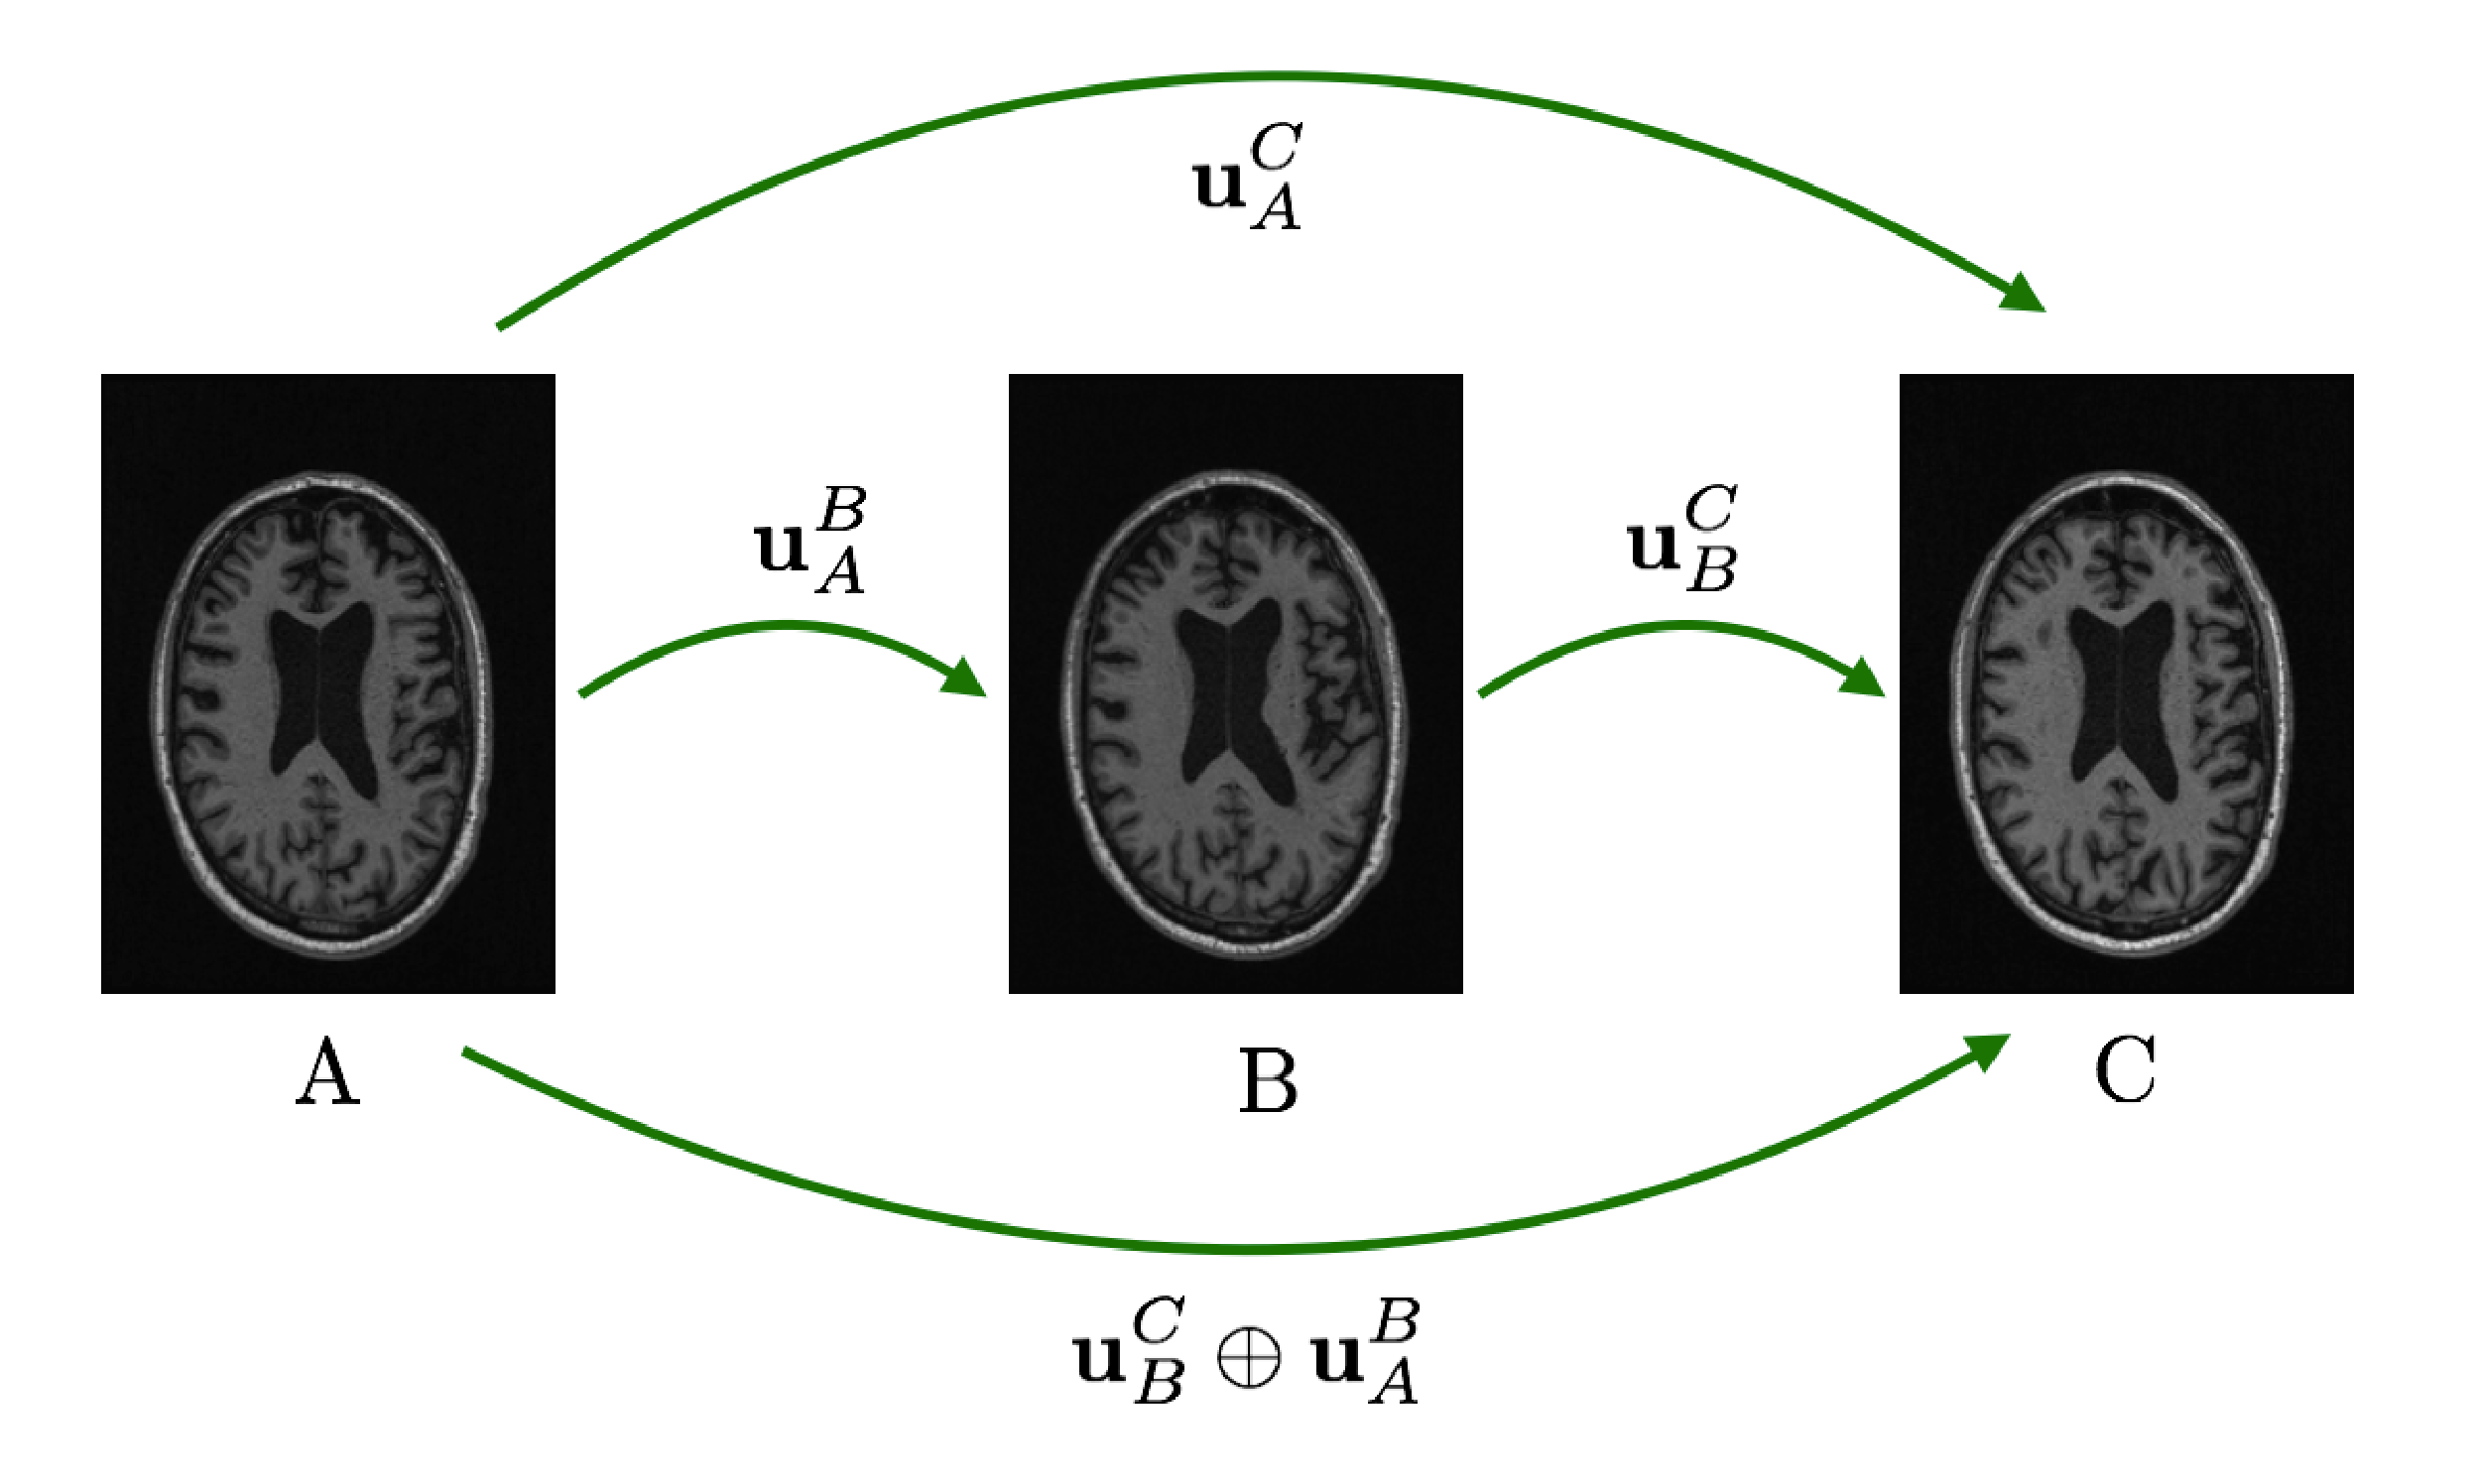
\includegraphics[scale=0.25]{figures/three_brains_problem.pdf}
	\caption{Design of the experiment with SVF obtained with real data. Three figures represents three  longitudinal scans of the same patient at time $A$, $B$ and $C$. The vector $\mathbf{u}_{A}^{B}$ is the SVF that corresponds to the non-rigid transformation from $A$ to $B$ that aligns the image $B$ with $A$. Equivalently $\mathbf{u}_{B}^{C}$ is the SVF from $B$ to $C$, and $\mathbf{u}_{A}^{C}$ from $A$ to $C$. For the ideal registration algorithm we have that $\log(\exp(\mathbf{u}_{B}^{C}) \circ \exp(\mathbf{u}_{A}^{B}))$ $=$ $\mathbf{u}_{A}^{C} $; when the first member is computed with a numerical method, the difference with the second member provides a measure of the error of the numerical method for the Lie log-composition. When the registration is not ideal, the equation (\ref{eq:error_real_data_formula}) provides a consistent measure of the error. }
	\label{fig:three_brains_problem}
\end{figure}

% % % % % % % % % % % % % % % % % % % % % % % % % % % % % % % % % % % % % %
\subsection{Design of Experiment}
We design a simple experiment that involves three T1 MRI longitudinal scans of the same subject in three points in time $A$, $B$ and $C$. $A$ is the baseline, $B$ is the first follow-up, and $C$ is the second follow-up.

Let $\varphi_{A}^{B}$ be the non-rigid transformation from $A$ to $B$ that aligns the image $B$ with $A$, $\varphi_{B}^{C}$ from $B$ to $C$ and $\mathbf{u}_{A}^{B}$, $\mathbf{u}_{B}^{C}$ the corresponding SVF.
Than for the analytic solution of the Lie log-composition, it follows that
\begin{align*}
	\exp(\alpha_0\mathbf{u}_{B}^{C} \oplus \alpha_1\mathbf{u}_{A}^{B})
	=
	\exp(\alpha_0\mathbf{u}_{B}^{C}) \circ\exp(\alpha_1\mathbf{u}_{A}^{B})
\end{align*} 
where $\alpha_0$ and $\alpha_1$ are two real numbers between $0$ and $1$ that are used to divide the norm of the considered SVF, by a percentage value.
Then we can use again the equation \ref{eq:error_svf_sythetic_data}, to compute the error of the numerical methods:
\begin{equation}
\begin{aligned}\label{eq:error_log_composition_real_data}
E^{M}(&\mathbf{u}_{A}^{B}, \mathbf{u}_{B}^{C}, p_0, p_1) = \\
&= 
\Big( \sum_{\mathbf{x} \in \Delta\Omega} 
\euclideanMetric{
	\exp(M(p_0\mathbf{u}_{B}^{C} \oplus p_1\mathbf{u}_{A}^{B}))(\mathbf{x}) 
	-
	\big(\exp(p_0\mathbf{u}_{B}^{C}) \circ\exp(p_1\mathbf{u}_{A}^{B})\big)(\mathbf{x}) 
}_{l^2}^{2}  \Big)^{1/2}
\end{aligned}
\end{equation}
After the computation, error is then normalized by the division for the square root of the product of the dimension of the $SVF$.

%% % % % % % % % % % % % % % % % % % % % % % % % % % % % % % % % % % % % % %
\subsection{Results}
%
The dataset has been collected from ADNI (Alzheimer Disease Neuroimaging Initiative) \cite{jack2008alzheimer} and consists of $3$ longitudinal scans of $16$ control subjects (CTL).
The baseline $A$ at time $0$ is followed by a first follow-up $B$, after three months, and a second follow up $C$, after $6$ months. The SVF of the transformations are obtained using NiftyReg. 

Figure \ref{fig:svf_log_composition_real_data_CTL_expo} shows the results of the equation (\ref{eq:error_log_composition_real_data}) where $M$ is one of the numerical methods based on $\text{BCH}^0$, $\text{BCH}^1$, $\text{BCH}^{1.5}$, $\text{BCH}^2$ and parallel transport (P.T.).
Axes indicates the values for $p_1$ and $p_0$, that corresponds to the following average norms of the $16$ SVF considered:

\begin{center}
 \begin{tabular}{ c | c | c | c | c | c  }
 	0.01 & 0.05 & 0.10 & 0.15 & 0.20 & 0.25 \\
 	\hline
 	 0.0045 &  0.0227 & 0.0454 & 0.0682 & 0.0909 & 0.1136
 \end{tabular}
\end{center}

Results are consistent with the one obtained for synthetic data except for the fact that when the norm of $\mathbf{u}_{A}^{B}$ si below $0.0227$ parallel transport method provides better results than the $\text{BCH}^1$. This can be explained by the fact that synthetic SVF with comparable norm have Jacobian determinant negative at some voxels, while for real data this does not happen. This would require a new method for generating synthetic SVF in which the positivity of the Jacobian determinant is assured.

Also in this case error obtained with $\text{BCH}^{1.5}$ and $\text{BCH}^2$ are not showed because they do not improve the numerical errors obtained with $\text{BCH}^1$, in particular for small SVF. 

\begin{figure}[!ht]
	\hspace{-1.0cm}
	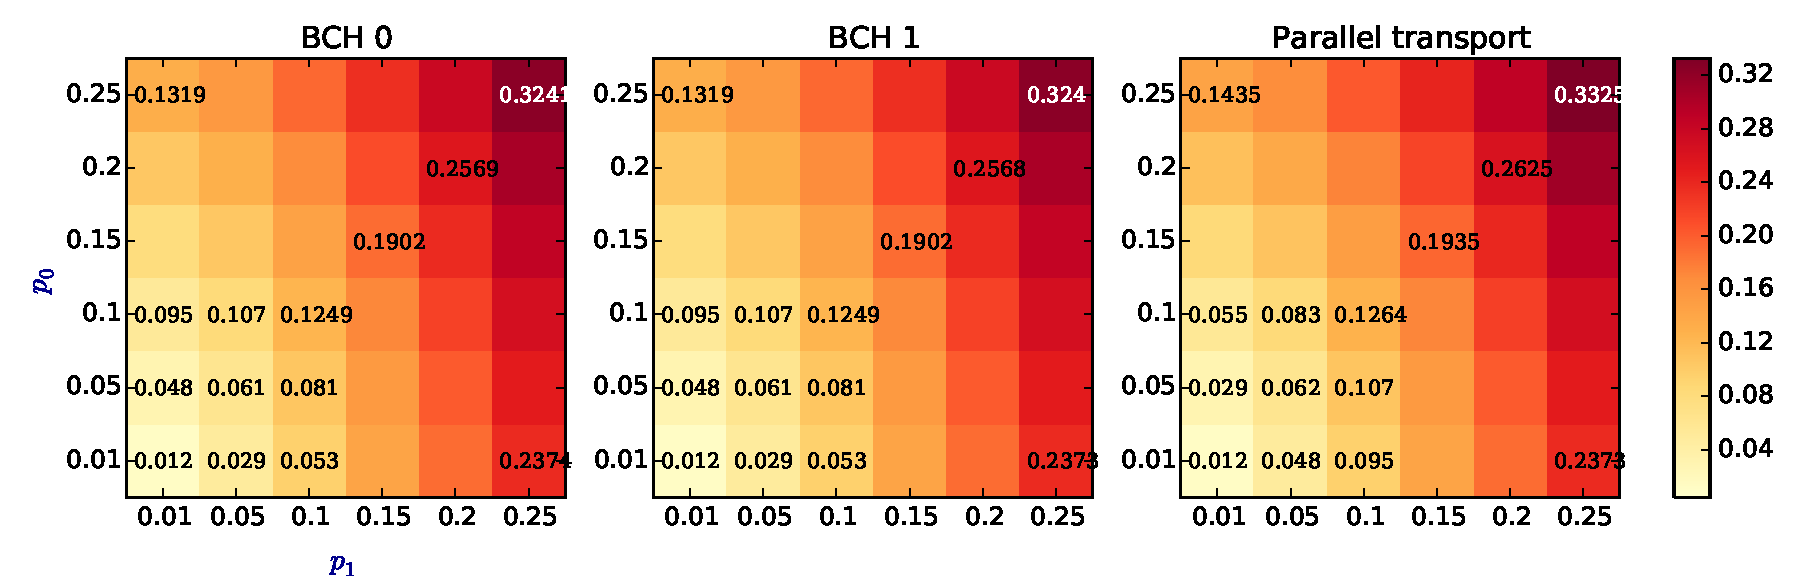
\includegraphics[scale=0.53]{figures/svf_log_composition_real_data_CTL_expo.pdf}
	\caption{Lie Log-composition errors for a dataset of 16 MRI T1 brain images scan of control subjects. Three longitudinal scans $A$, $B$ and $C$ are available for each subject, and corresponds to a scan at time $0$, after three months and after $6$ month from the $0$. The design of the experiment is shown in figure \ref{fig:three_brains_problem}, and the error of the Lie log-composition is computed with the formula (\ref{eq:error_log_composition_real_data}).}
	\label{fig:svf_log_composition_real_data_CTL_expo}
\end{figure}


% % % % % % % % % % % % % % % % % % % % % % % % % % % % % % % % % % % % % %
% % % % % % % % % % % % % % % % % % % % % % % % % % % % % % % % % % % % % % 
% % % % % % % % % % % % % % % % % % % % % % % % % % % % % % % % % % % % % % 
\section{Lie Logarithm computation for $SE(2)$}\label{se:results_lie_logarithm_computations}

This section is devoted the results of the numerical methods developed in chapter \ref{ch:log_algorithm}. Different numerical methods for the computation of the Lie logarithm are compared when a ground truth is available, i.e. in the finite dimensional case. We consider a data set of $200$ random matrices in the Lie group $SE(2)$ with their respective logarithm in $\mathfrak{se}(2)$ computed using the closed form presented in chapter \ref{ch:spatial_transformations}. 

For each of the method considered and for each of the random matrix we always have convergence up to a precision of $10^{-12}$ before the $20^{\text{th}}$ iteration.
In particular, in figure \ref{fig:log_computation_boxplot} we can see the average number of iterations required to reach the solution with a precision of $10^{-4}$ for each of the numerical method considered. Each box represents $200$ random matrices in $SE(2)$ with Frobenius norm uniformly selected between $1$ and $3$.

As obtained for the numerical computations of the Lie log-composition, results obtained with parallel transport are comparable with the results obtained with the truncated BCH of degree $1$. Also in this case, an increase in the degree of the truncated BCH does not ensure a faster convergence and the Taylor method provides the slowest algorithm. The reason for this fact is not clear are the moment and, excluding errors, it may be worthed to future investigations.

\begin{figure}[!ht]
	\hspace{-0.5cm}
	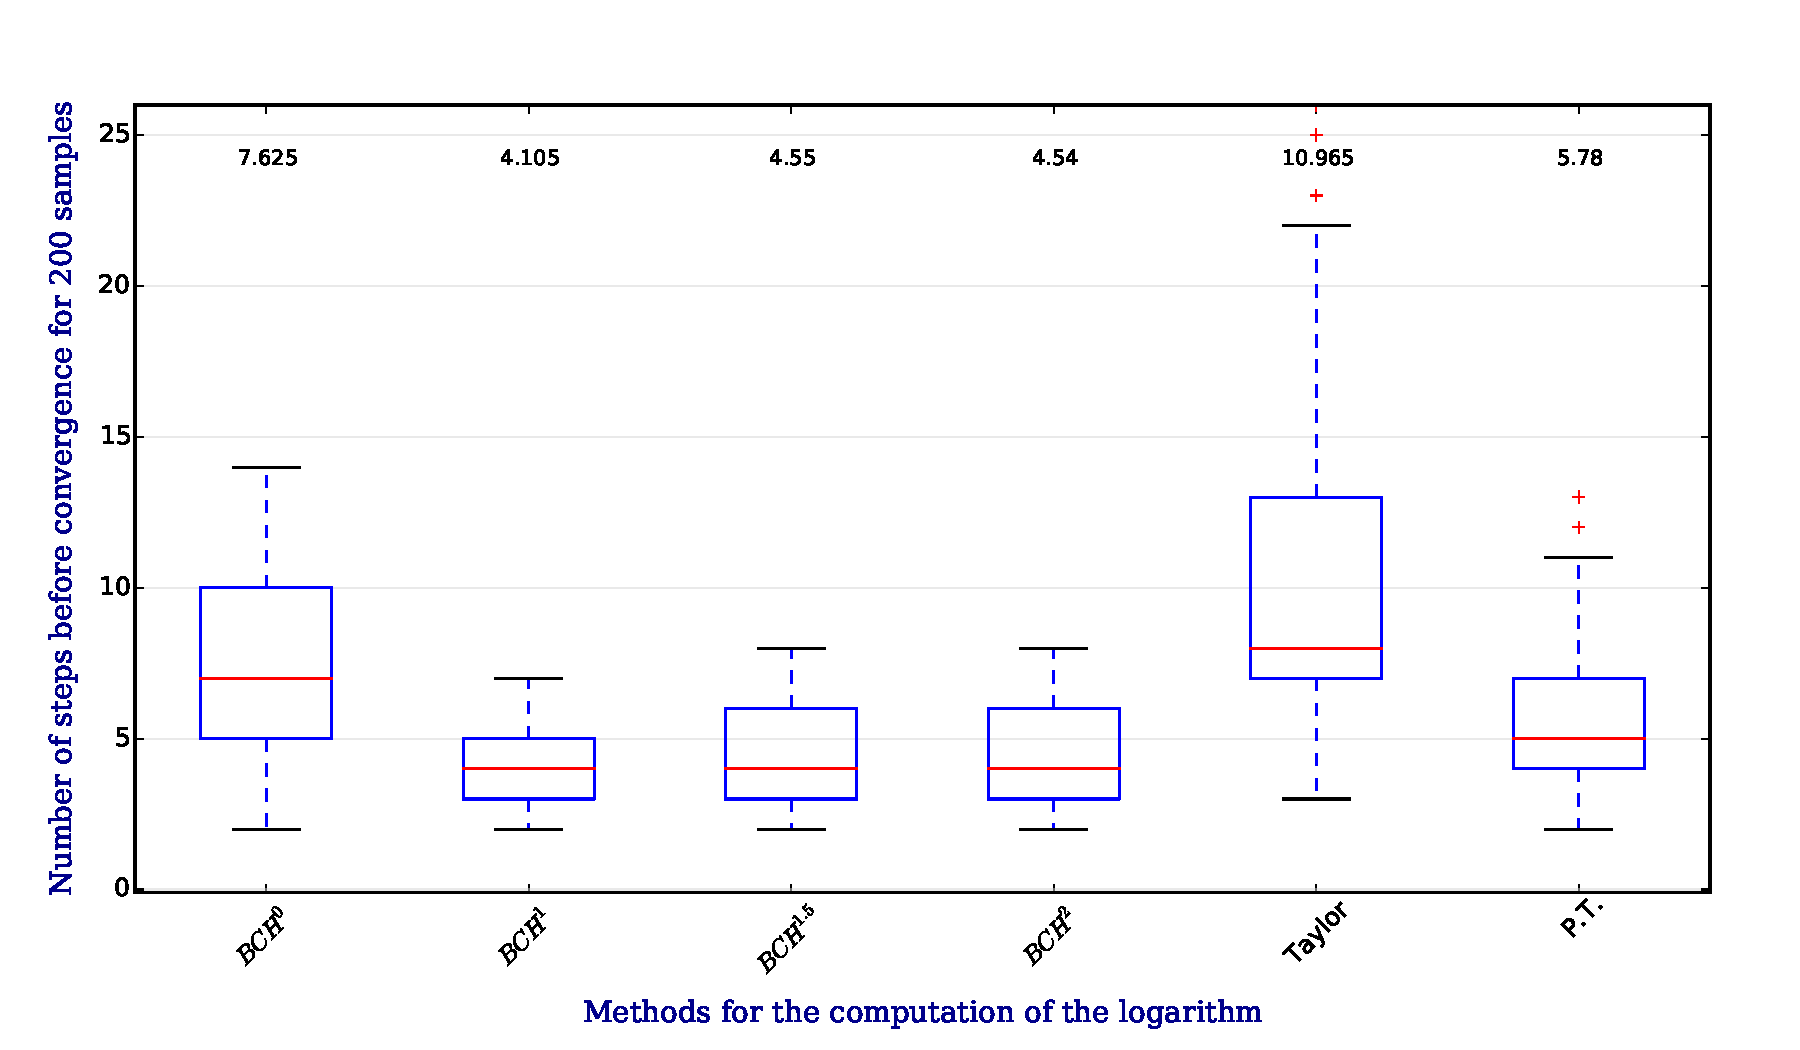
\includegraphics[scale=0.5]{figures/log_computation_boxplot.pdf}
	\caption{Number of steps required to obtain convergence for different methods utilized in the logarithm computation algorithm. The data set contains $200$ random matrices in the Lie group $SE(2)$, with Frobenius norm between $1$ and $3$. On the top it is possible to visualize the mean number of step to reach the convergence for each method.}
	\label{fig:log_computation_boxplot}
\end{figure}


% % % % % % % % % % % % % % % % % % % % % % % % % % % % % % % % % % % % % %
% % % % % % % % % % % % % % % % % % % % % % % % % % % % % % % % % % % % % % 
\section{Empirical Evaluations of the Computational Time}

Last results here proposed are an empirical evaluation of the computational time. 
For the finite dimensional case, a dataset of $36000$ random generated matrix with norm between $0.0$ and $2.0$ has been utilized to measure the empirical computational time of each of the numerical methods for the computation of the log-composition here presented. Computations are performed with a Mac book pro 2014, 16Gb Ram. Sum of the computational time for the whole data set are give in seconds:\\

\hspace{-1cm}
\begin{tabular}{ c | c | c | c | c | c | c }
Ground & $\text{BCH}^0$ & $\text{BCH}^1$ & $\text{BCH}^{1.5}$ & $\text{BCH}^2$ & Taylor & p.t. \\
\hline
1.07402015 & 0.18845153 & 0.57751322 & 1.24413943 & 1.78752184 & 0.77354765 &
2.26586294 
\end{tabular}
\vspace{0.5cm}

The first column provides the computational time of the ground truth, i.e. the time to compute the closed form for the computation of $dr_0 \oplus dr_{1}$. As expected the burden time to compute the $\text{BCH}^0$ for a dataset of size $36000$, is the lowest since it consists simply in a sum, while the computation of the parallel transport is four time slower than the $\text{BCH}^1$, since it involves three times the computation of the Lie exponential and two times the resampling.

When dealing with SVF, the computational time strongly depends on the size of the vector field involved. In figure \ref{fig:svf_computational_time} we show the relations between the size of the vector field and the increase in the computational time for a data set of $20$ random generated SVF.

\begin{figure}[!ht]
	%\hspace{-0.5cm}
	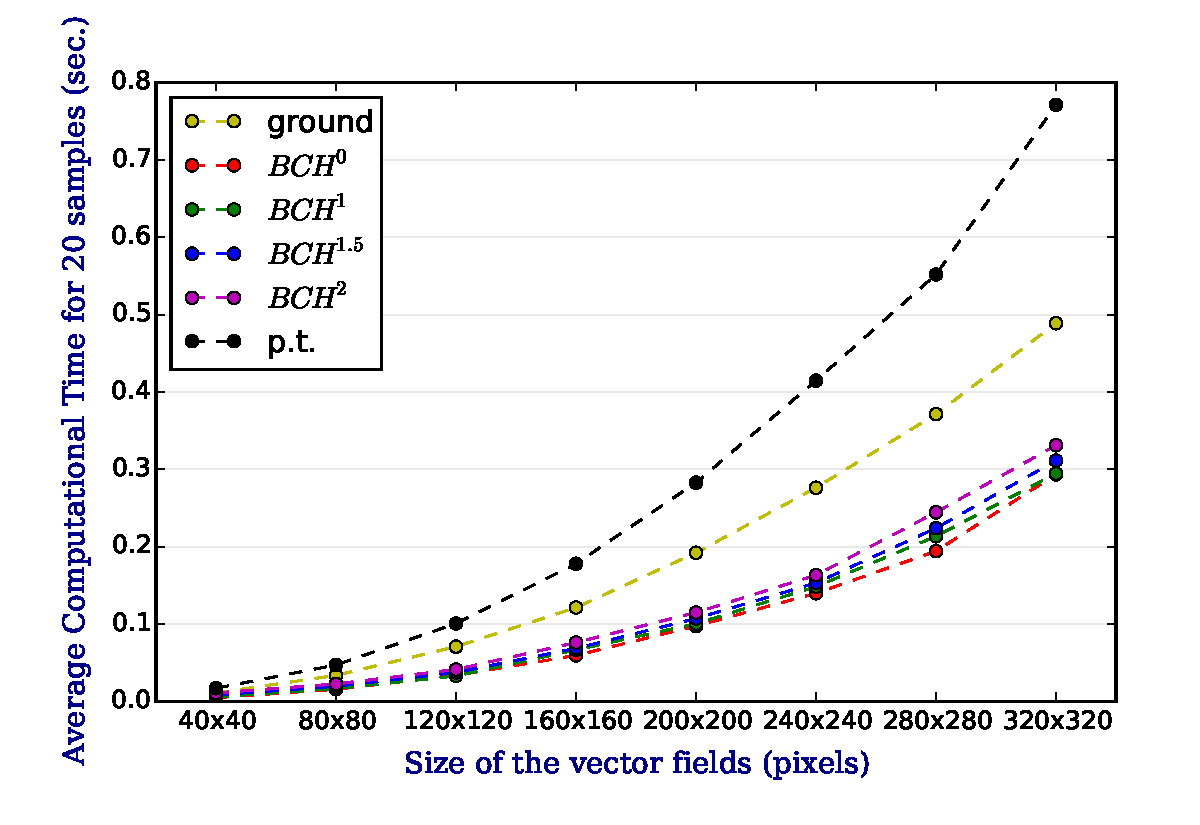
\includegraphics[scale=0.7]{figures/svf_computational_time.pdf}
	\caption{Relationships between the size of the figure (x-axes) and the computational time for a data set of $20$ random generated SVF. The yellow line labeled with ground represents the time of the computation of $\exp{\mathbf{u}_0}\circ \exp{\mathbf{u}_1}$, while the other represents the exponentiation of the numerical method for the computation of the log-composition.}
	\label{fig:svf_computational_time}
\end{figure}




%% theoretical side in general
%Starting from the definition of Lie log-group of diffeomorpshisms $(\mathfrak{g} , \oplus)$, to have an algebraic definition of this approximation, we can consider its quotient over the ideal generated by $(\text{ad}_{\mathbf{u}}^{m}, \text{ad}_{\mathbf{u}}^{n})$, which provides the group $(\quotient{\mathfrak{g}}{(\text{ad}_{\mathbf{u}}^{m}, \text{ad}_{\mathbf{u}}^{n})}, \oplus)$. Further investigations in this direction is not prosecuted.


% OLD EXPERIMENT:
%
%then for an ideal registration algorithm (that fully satisfies the transitivity property) we have
%\begin{align}\label{eq:transitivity_of_the_registration}
%\varphi_{B}^{C} \circ \varphi_{A}^{B} = \varphi_{A}^{C}  
%\end{align}
%From this assumption, it follows:
%\begin{align*}
%\log(\varphi_{B}^{C} \circ \varphi_{A}^{B}) &= \log(\varphi_{A}^{C}  ) \\
%\log(\exp(\mathbf{u}_{B}^{C}) \circ \exp(\mathbf{u}_{A}^{B})) &= \log(\exp(\mathbf{u}_{A}^{C}  ) ) \\
%\log(\exp(\mathbf{u}_{B}^{C}) \circ \exp(\mathbf{u}_{A}^{B})) &= \mathbf{u}_{A}^{C}  
%\end{align*}
%The exact solution of the log-composition would provide then:
%\begin{align*}
%\int_{\Omega} \euclideanMetric{
%	\mathbf{u}_{B}^{C} \oplus \mathbf{u}_{A}^{B}
%	-
%	\mathbf{u}_{A}^{C}
%}_{L^2}^{2} d\mathbf{x} 
% =
% 0
%\end{align*} 
%While, when $\mathbf{u}_{B}^{C} \oplus \mathbf{u}_{A}^{B}$ is approximated with some numerical method $M$, the previous integral provides its error.
%\begin{align}\label{eq:error_real_data_formula} 
%\int_{\Omega} \euclideanMetric{
%	M\big(\mathbf{u}_{B}^{C} \oplus \mathbf{u}_{A}^{B} \big)
%	-
%	\mathbf{u}_{A}^{C}
%}_{L^2}^{2} d\mathbf{x} 
%=
%\text{Error}_{\oplus}
%\end{align} 
%
%Certainly, the equation (\ref{eq:transitivity_of_the_registration}) is correct only for the ideal registration algorithm, and the distance between the two members, computed using for example the metric $d^{1}$ defined in equation (\ref{def:metric_two_displacement_field}) is different from zero in real applications:
%\begin{align*}
%d^{1}(\varphi_{B}^{C} \circ \varphi_{A}^{B} ,\varphi_{A}^{C}) 
%= 
%\text{Error}_{\text{reg}}
%\end{align*} 
%But the error $\text{Error}_{\text{reg}}$ has the same effect for all of the numerical methods that approximate the log-composition. Therefore, even if the equation (\ref{eq:error_real_data_formula}) does not measures exclusively the numerical error of the Lie log-composition, its result is consistent for different numerical methods.
%
%% % % % % % % % % % % % % % % % % % % % % % % % % % % % % % % % % % % % % %
%\subsection{Results}
%
%The dataset has been collected from ADNI (Alzheimer Disease Neuroimaging Initiative) \cite{jack2008alzheimer} and consists of $3$ longitudinal scans of $16$ control subjects (CTL).
%The baseline $A$ at time $0$ is followed by a first follow-up $B$, after three months, and a second follow up $C$, after $6$ months.
%
%\begin{figure}[!ht]
%	\hspace{-1.0cm}
%	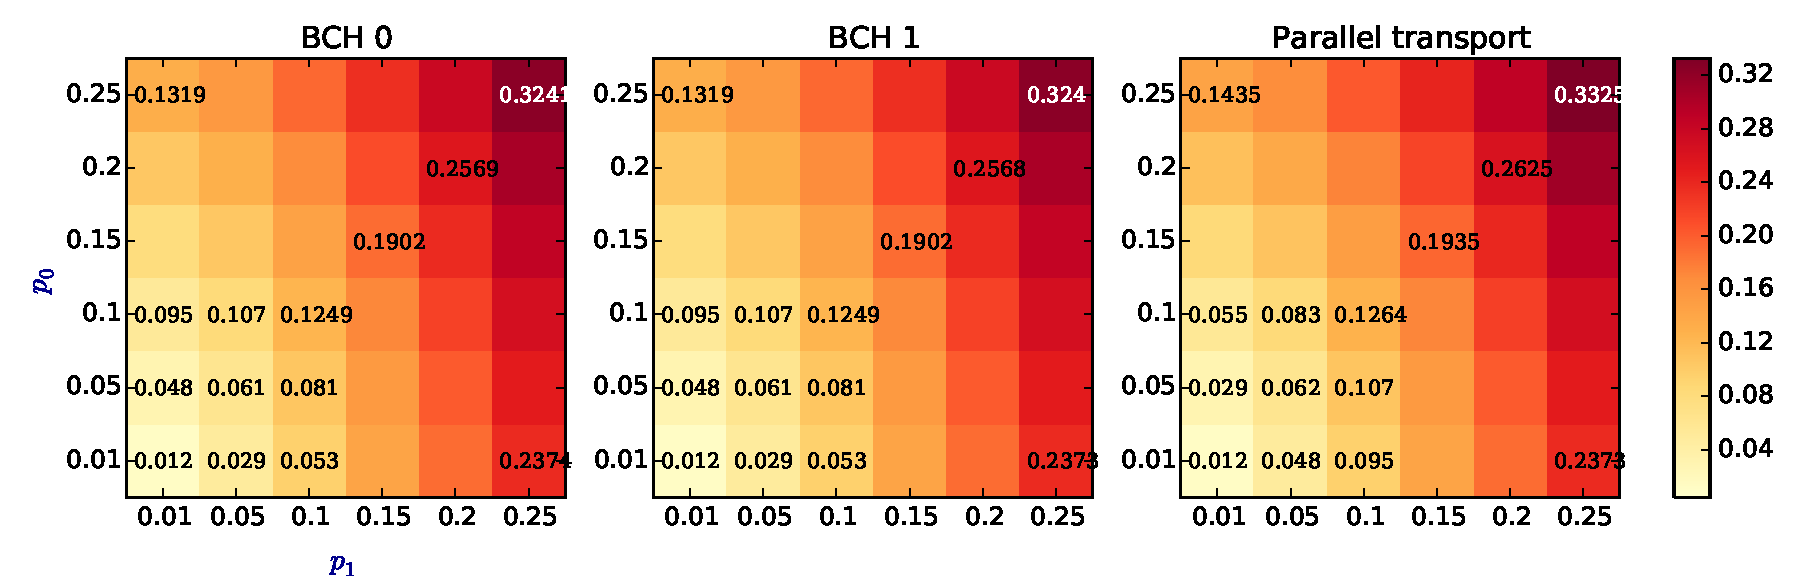
\includegraphics[scale=0.5]{figures/svf_log_composition_real_data_CTL_expo.pdf}
%	\caption{Lie Log-composition errors for a dataset of 16 MRI T1 brain images scan of control subjects. Three longitudinal scans $A$, $B$ and $C$ are available for each subject, and corresponds to a scan at time $0$, after three months and after $6$ month from the $0$. The design of the experiment is shown in figure \ref{fig:three_brains_problem}, and the error of the Lie log-composition is computed with the formula (\ref{eq:error_real_data_formula}).}
%	\label{fig:svf_log_composition_real_data_CTL_expo}
%\end{figure}
%
%The SVF of the transformations are obtained using NiftyReg by the non-rigid registration algorithm based on cubic B-spline. 
%
%Figure \ref{fig:svf_log_composition_boxplot_real_data_CTL} shows the results of the equation (\ref{eq:error_real_data_formula}) where $M$ is one of the numerical methods based on $\text{BCH}^0$, $\text{BCH}^1$, $\text{BCH}^{1.5}$, $\text{BCH}^2$ and parallel transport (P.T.). Results are consistent with the one obtained for synthetic data. The error obtained with the Parallel transport method is between $\text{BCH}^0$ and $\text{BCH}^1$, while an increase in the degree of the truncated BCH does no imply on the average a better approximation of the log-composition. For real applications is not recommendable to utilize $\text{BCH}^k$ for $k\geq 2$. The best method is the $\text{BCH}^1$ that involves one nested Lie bracket, while the parallel transport is the first choice (and the unique at the moment) when it is preferable to avoid the computation of the Lie bracket. 





